%%% File: ./inputs/NEUROSCIENCE.tex

%%% %%%%%%%%%%%%%%%%%%%%%%%%%%%%%%%%%%%%%%%%%%%%%%%%%%%%%%%%%%%%%%%%%%%%%%%%%%%%

\section{Neuroscience}
\label{section_neuroscience}

%%% %%%%%%%%%%%%%%%%%%%%%%%%%%%%%%%%%%%%%%%%%%%%%%%%%%%%%%%%%%%%%%%%%%%%%%%%%%%%

%%% \begin{quotation}
%%% %
%%%   Neuroscience offers a rich source of ideas relating to human cognition. The challenge for researchers working in machine learning and artificial intelligence is to translate those ideas into useful technologies. Increasingly, the technologies these researchers are developing are playing an important role in accelerating neuroscience by providing useful tools and models. There are significant opportunities for much closer cooperation between the different fields, but they require effort on both sides. The next section offers a sample of ideas drawn from neuroscience that are influencing our work.
%%% %
%%% \end{quotation}
  
%%%  This paper describes the focus, content and products of an advanced class in computational neuroscience at Stanford University. The focus is on the intersection between neuroscience and artificial intelligence. The content varies but for the last two years has emphasized cognitive architectures for digital agents like the programmer's apprentice. The products of the class are ideas, contacts and aspirations: ideas at the bleeding edge of neuroscience and artificial inteligence and the context in which to understand and apply them; contacts with scientists from around the world who talk about their work and lead discussions about what's new and next; and asprations to build the next generation of tools and technologies leveraging ideas from neuroscience and artificial intelligence.

From the brain of an Etruscan shrew weighing in at less than a tenth of a gram to a sperm whale brain weighing more than eight kilograms, it is clear that natural selection has stumbled on a basic brain plan and set of developmental strategies that enables it to construct a diverse set of special-purpose brain architectures for efficiently expressing a wide range of sophisticated behavior~\cite{DouglasandMartinCURRENT-BIOLOGY-12,WillemetBRAIN-SCIENCE-12}. The human brain with its approximately 100 billion neurons and the shrew brain with approximately 1 million neurons share the same basic architecture.

The mouse brain has homologues of most human subcortical nuclei and has contributed significantly to our understanding of the human brain and human neurodegenerative disease in particular. The differences between between human and chimpanzee brains are subtle~\cite{Mora-BermudezetalELIFE-16} and yet humans display a much wider range of behavior and express a much larger repertoire of genes than any other species~\cite{HawrylyczetalNATURE-NEUROSCIENCE-15}. So what makes the difference?

It's the connections between neurons that matter or, more generally, it's the different types of communication between neurons that biologists refer to as {\it{pathways}}. There are electrical, chemical and genetic pathways and each of them obey different constraints and are used for different purposes. They include point-to-point and broadcast methods of communication~\cite{HanetalNATURE-18}. They transfer information at different speeds and using different coding strategies. Layered architectures are common not just in the cortex but throughout the brain. It's the wiring that sets humans apart.

%%% %%%%%%%%%%%%%%%%%%%%%%%%%%%%%%%%%%%%%%%%%%%%%%%%%%%%%%%%%%%%%%%%%%%%%%%%%%%%

% DISTRIBUTED FUNCTION
\subsection{Connectivity}

%%% %%%%%%%%%%%%%%%%%%%%%%%%%%%%%%%%%%%%%%%%%%%%%%%%%%%%%%%%%%%%%%%%%%%%%%%%%%%%

%%% Figure~{\urlh{#fig_Human_Brain_Neocortex_Function}{\ref{fig_necortex}}}
\begin{figure}
%
  \begin{center} 
%    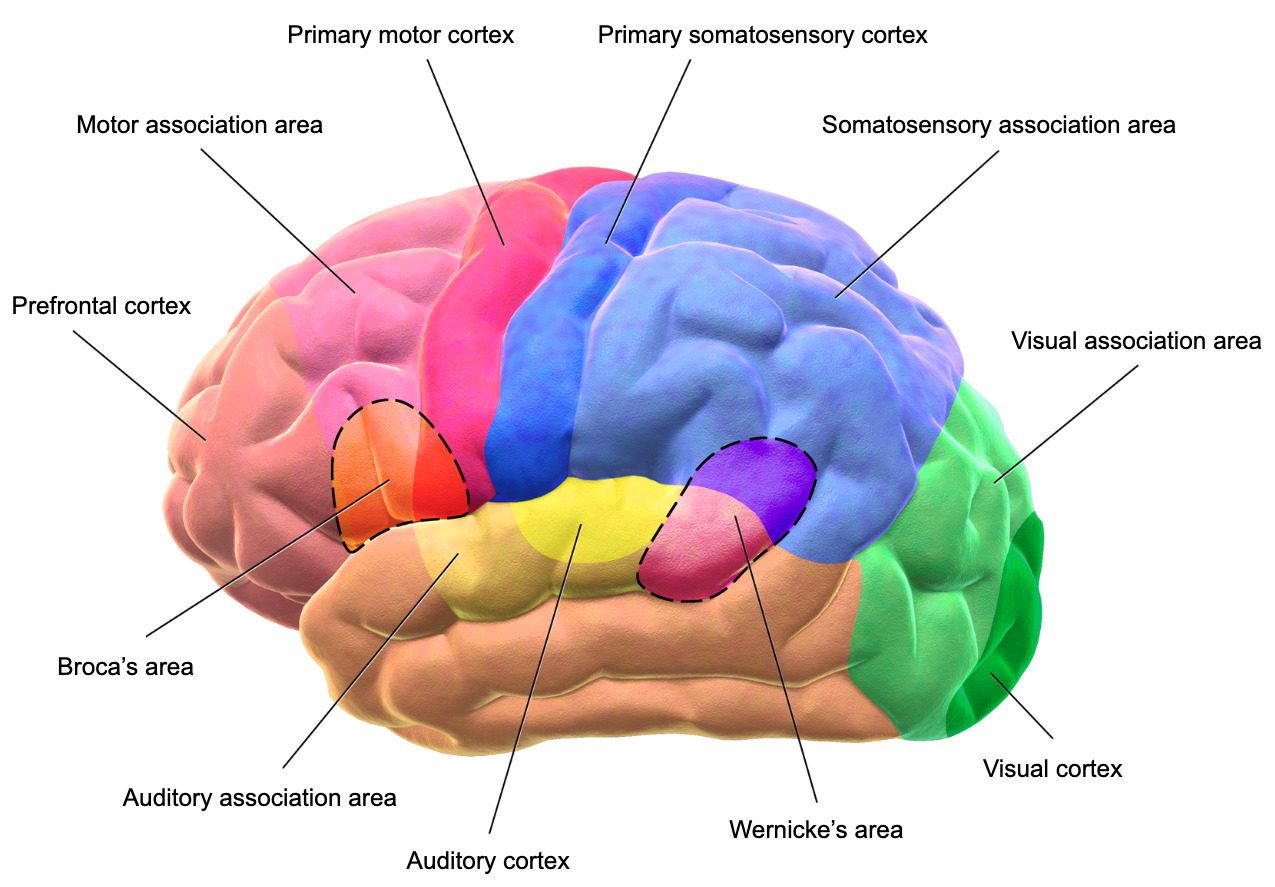
\includegraphics[height=600pt]{./figures/Human_Brain_Neocortex_Function.png} 
    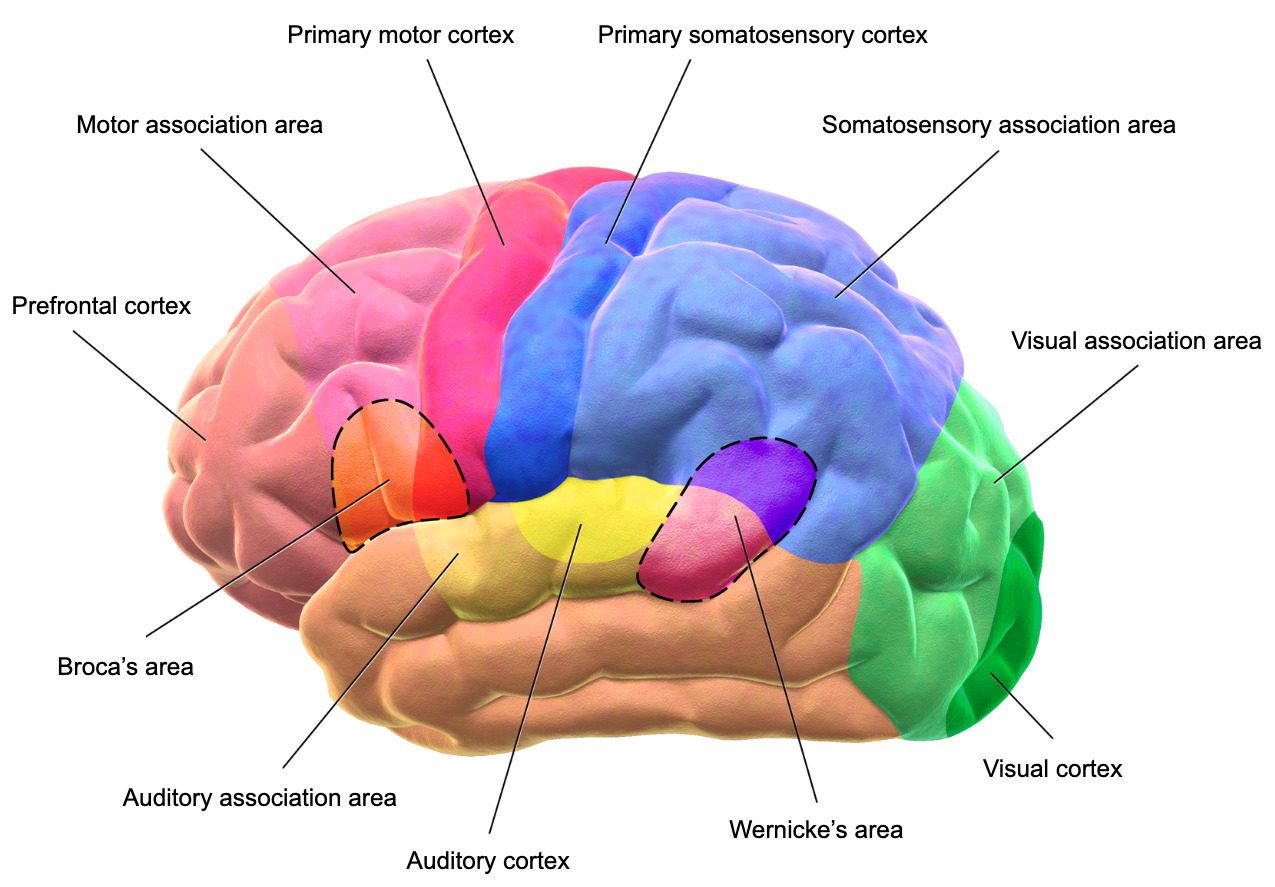
\includegraphics[height=200pt]{./figures/Human_Brain_Neocortex_Function.png} 
  \end{center}
%
  \caption{A highly stylized rendering of the major functional areas of the human cortex shown from the side with the head facing to left. Highlighted regions include the occipital lobe shown in shades of green including the primary visual cortex; the parietal lobe shown in shades of blue, including the primary somatosensory cortex; the temporal lobe shown in shades of yellow including the primary auditory cortex; and the frontal lobe shown in shades of pink, including the primary motor and prefrontal cortex. The region outlined by a dashed line on the left is Broca's area and it is historically associated with the production of speech and hence its position relative to the motor cortex. The region outlined by a dashed line on the right is Wernicke’s area and it is historically associated with the understanding of speech and hence its position relative to the sensory cortex. Broca's and Wernicke's areas are found only in the dominant hemisphere which is usually the left as shown here.}
%%%  \caption{A highly stylized rendering of the major functional areas of the human cortex shown from the side with the head facing to right. Highlighted regions include the occipital lobe shown in shades of green including the primary visual cortex; the parietal lobe shown in shades of blue, including the primary somatosensory cortex; the temporal lobe shown in shades of yellow including the primary auditory cortex; and the frontal lobe shown in shades of pink, including the primary motor and prefrontal cortex. The region outlined by a dashed line on the right is Broca’s area and it is historically associated with the production of speech and hence its position relative to the motor cortex. The region outlined by a dashed line on the left is Wernicke’s area and it is historically associated with the understanding of speech and hence its position relative to the sensory cortex.}
%
  \label{fig_necortex}
%
\end{figure}

%%% %%%%%%%%%%%%%%%%%%%%%%%%%%%%%%%%%%%%%%%%%%%%%%%%%%%%%%%%%%%%%%%%%%%%%%%%%%%%


%%% %%%%%%%%%%%%%%%%%%%%%%%%%%%%%%%%%%%%%%%%%%%%%%%%%%%%%%%%%%%%%%%%%%%%%%%%%%%%

Figure~{\urlh{#fig_Human_Brain_Neocortex_Function}{\ref{fig_necortex}}} shows the major functional areas of the human neocortex including the primary and secondary sensory and motor areas. The proximal locations of the areas provide a very rough idea of how different functions might relate to another. The graphic shown belies the fact that the brain is three dimensional and much of its functional circuitry hidden under the cortical sheet. The human cerebral cortex is complexly folded to fit within the skull with much of it hidden within the folds. This folded sheet of tissue accounts for more than 75\% of the human brain by volume~\cite{SwansonTiN-95} and is largely responsible for the rich behavioral repertoire that humans exhibit. It is worth pointing out in this context that the cortical sheet enshrouds a collection of evolutionarily preserved and highly specialized circuits homologues of which are found in all mammals and without which the cortex would be useless.

The graphic shown in Figure~{\urlh{#fig_Human_Brain_Neocortex_Function}{\ref{fig_necortex}}} is a simplification of the standard medical textbook diagram. In particular, several of the association areas are not shown and those that are shown are labeled somewhat differently than is common practice. The organizing biological principle is that, the further away from the primary sensory areas, associative functions become more general by integrating information from multiple modalities to construct abstract representations tailored to serve ecologically relevant objectives~\cite{Higher_Cortical_Functions_Association}. It is worth contemplating the arrangement of areas to note that they converge on locations in the cortex that will play an important role in decision making and higher-order cognition more generally.

%%% %%%%%%%%%%%%%%%%%%%%%%%%%%%%%%%%%%%%%%%%%%%%%%%%%%%%%%%%%%%%%%%%%%%%%%%%%%%%

%%% Figure~{\urlh{#fig_Human_Brain_Atlas_Allen_Institute}{\ref{fig_brains}}}
\begin{figure}
%
  \begin{center} 
%    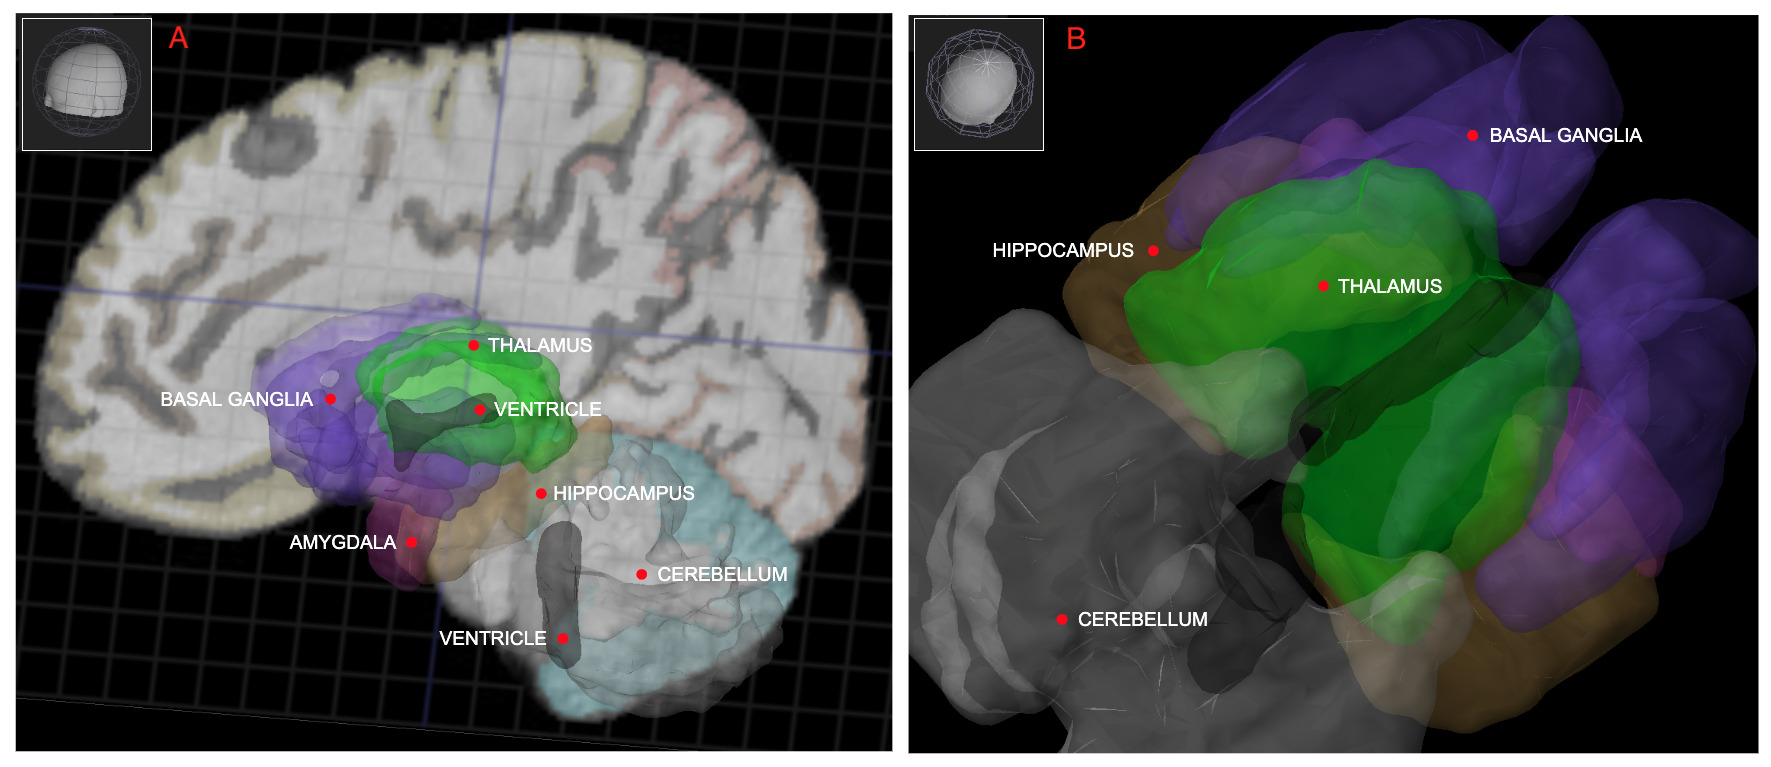
\includegraphics[height=600pt]{./figures/Human_Brain_Atlas_Allen_Institute.png} %%% 1806 × 799 pixels
    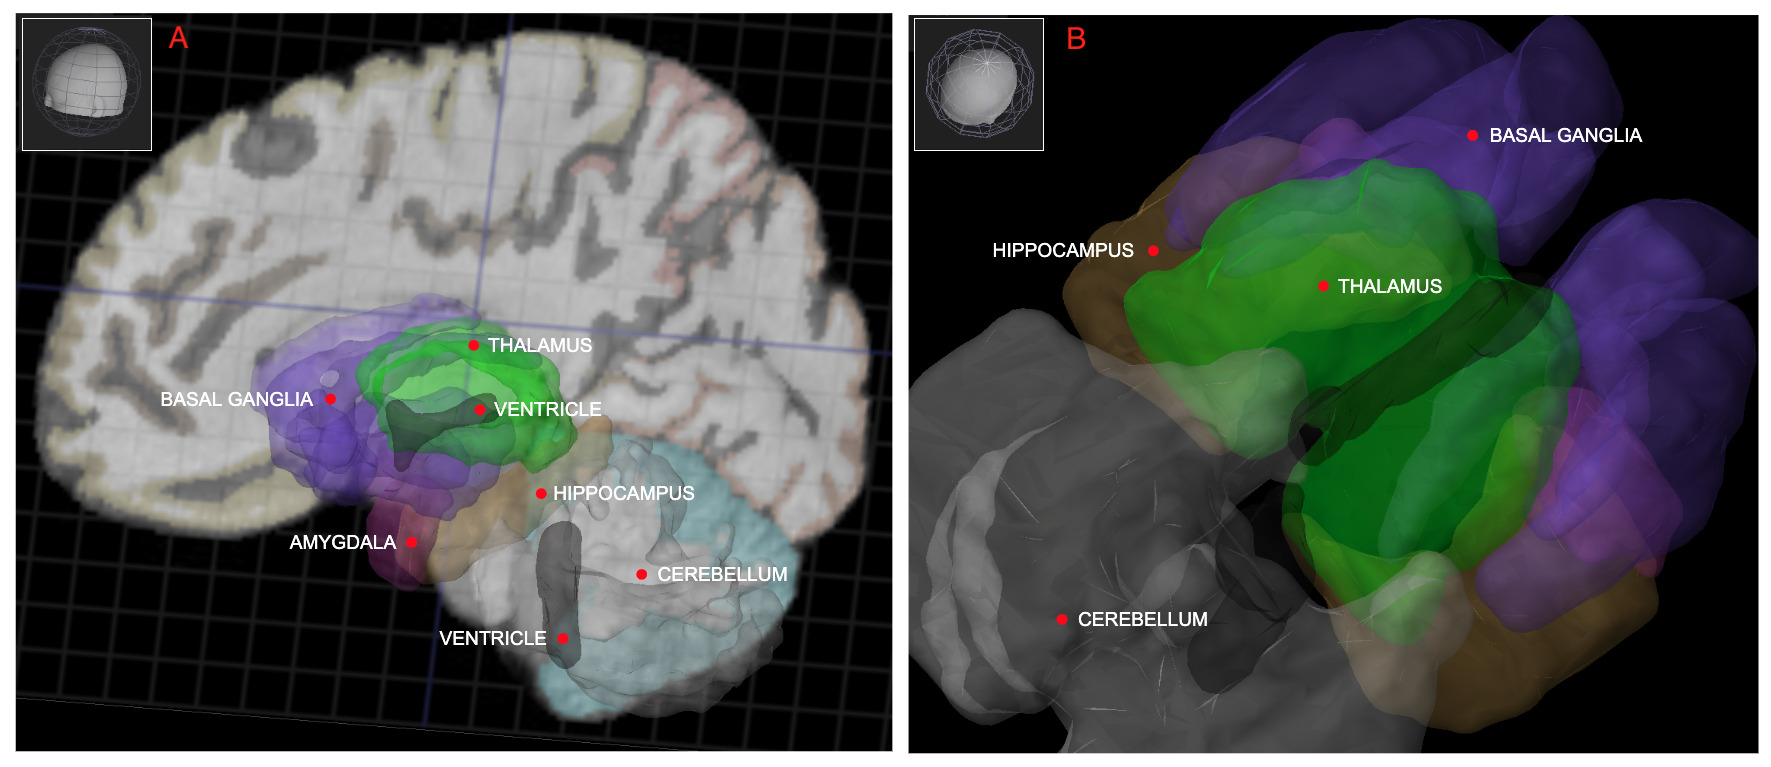
\includegraphics[height=150pt]{./figures/Human_Brain_Atlas_Allen_Institute.png} %%% 1806 × 799 pixels
  \end{center}
%
  \caption{Two 3-D renderings of the human brain generated by the Allen Institute {\urlh{ttp://human.brain-map.org/static/brainexplorer}{Brain Explorer}} from the Allen Human Brain Reference Atlas~\cite{HawrylyczetalNATURE-12}. The inset shown in the left upper corner of each panel indicates the orientation of the head. The left panel ({\colorred{A}}) shows 3-D reconstructions of several subcortical nuclei featured in this paper. A cross-sectional view of the whole brain is projected on the mid-sagittal plane dividing the right and left sides of the brain illustrating how the cortex envelopes the subcortical regions. The right panel ({\colorred{B}}) shows the same subcortical nuclei as seen from above (horizontal plane) and to the rear of the brain illustrating how the thalamus is located between the cortical sheet and the subcortical nuclei serving in its role as a relay between the two regions.}
%
  \label{fig_brains}
%
\end{figure}

%%% %%%%%%%%%%%%%%%%%%%%%%%%%%%%%%%%%%%%%%%%%%%%%%%%%%%%%%%%%%%%%%%%%%%%%%%%%%%%

Figure~{\urlh{#fig_Human_Brain_Atlas_Allen_Institute}{\ref{fig_brains}}} highlights the 3-D structure of several subcortical nuclei emphasized in this paper showing how they relate anatomically to one another and to the cortex. The reconstructions were generated from data generated by {\it{functional magnetic resonance imaging}} (fMRI) of adult human subjects~\cite{HawrylyczetalNATURE-12} and offer additional functional insight complementing conventional histological studies~\cite{BridgeandClarePTRS-B-06}. They don't however provide detailed information concerning either local or long-range connectivity.

Traditionally, tracing connections between individual neurons has been accomplished using a variety of techniques including conventional histological and staining techniques, electrophysiology, neurotropic retroviruses and transgenic organisms expressing fluorescent proteins. However, these methods yield relatively sparse reconstructions and don't scale well to large tissue samples~\cite{Arenkiel2014neural,CallawayCURRENT-OPINION-08}.

Small samples of neural tissue can be fixed, stained and sliced into thin sections. Each of the sections is then scanned with an electron microscope and the resulting digital images analyzed with computer vision software to reconstruct neurons and identify synapses~\cite{MikulaandDenkNATURE-METHODS-15}. The process is time consuming but can be fully automated and scaled to handle larger samples~\cite{JanuszewskietalNATURE-METHODS-18,ZhengetalCELL-18}. 

It is also possible to reconstruct the major {\it{white matter tracts}} formed by bundles of myelinated fibers using diffusion-weighted fMRI and averaging over multiple subjects after registering the individual brain scans with a reference atlas~\cite{OishietalNEUROIMAGE-08,WakanaetalRADIOLOGY-04}. Unlike the previous technologies, this method is not destructive so it can be applied to human subjects and accuracy is improved by averaging over multiple subjects after registering the individual brain scans with a reference atlas

These major tracts increase the speed of signal transmission between regions allowing for more distant communication in larger brains. The differences between the neocortex in humans and chimpanzees are subtle~\cite{Mora-BermudezetalELIFE-16}; however, white matter connections observed in humans but not in chimpanzees particularly link multimodal areas of the temporal, lateral parietal, and inferior frontal cortices, including tracts important for language processing~\cite{ArdeschetalPNAS-19,Gomez-RoblesetalPNAS-15}.

%%% %%%%%%%%%%%%%%%%%%%%%%%%%%%%%%%%%%%%%%%%%%%%%%%%%%%%%%%%%%%%%%%%%%%%%%%%%%%%

%%% Figure~{\urlh{#fig_White_Matter_Tracts_Long_Distance}{\ref{fig_tracts}}}
\begin{figure}
%
  \begin{center} 
%    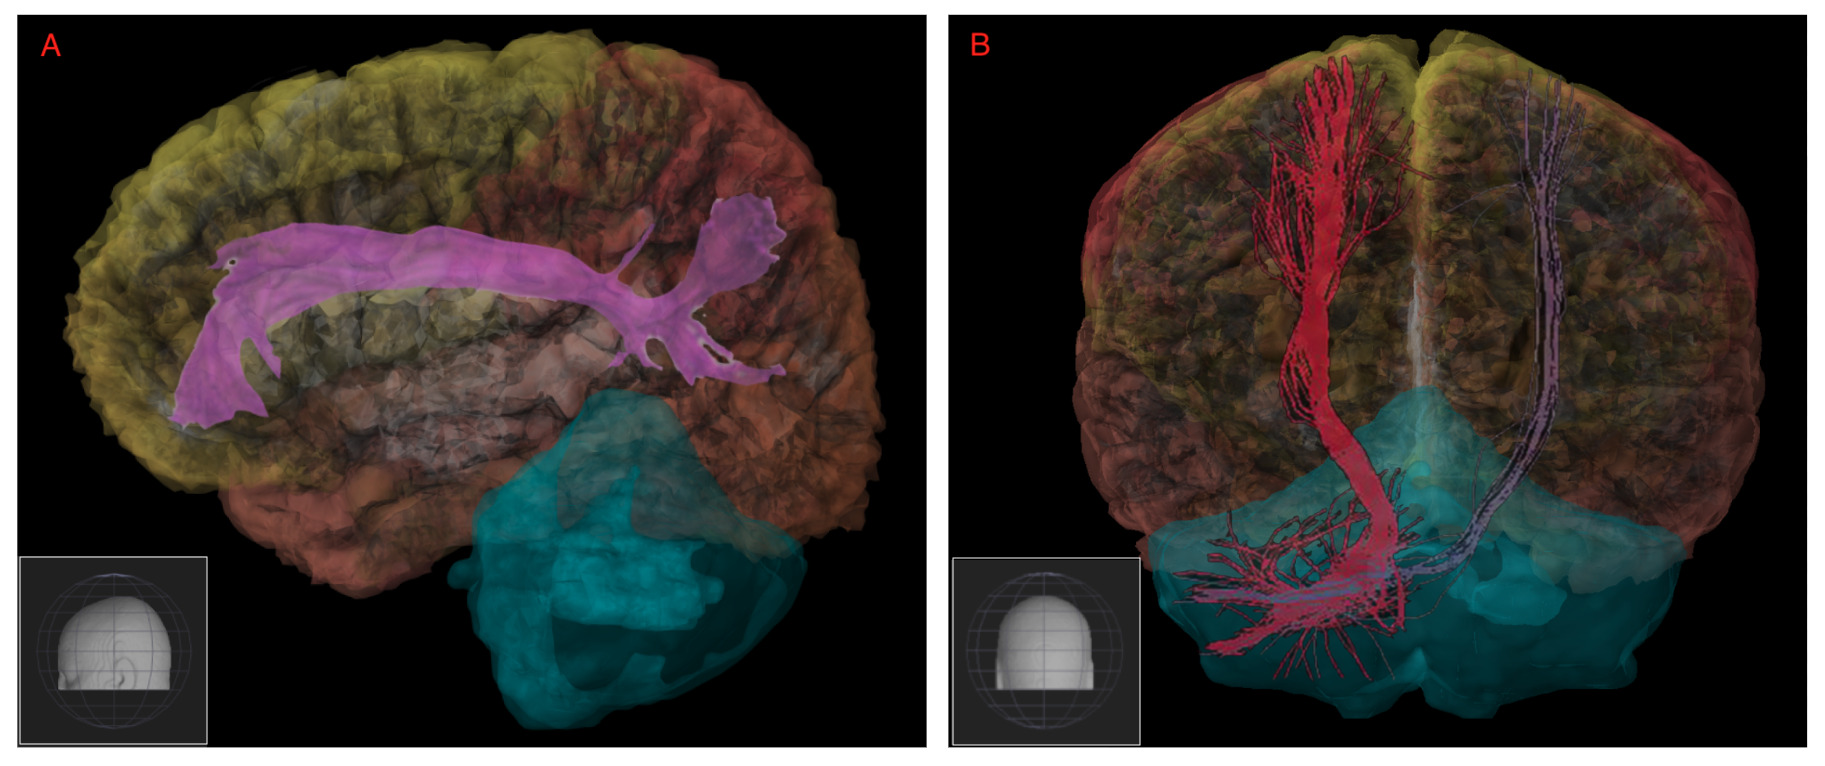
\includegraphics[height=600pt]{./figures/White_Matter_Tracts_Long_Distance.png} %%% 1873 × 810 pixels
    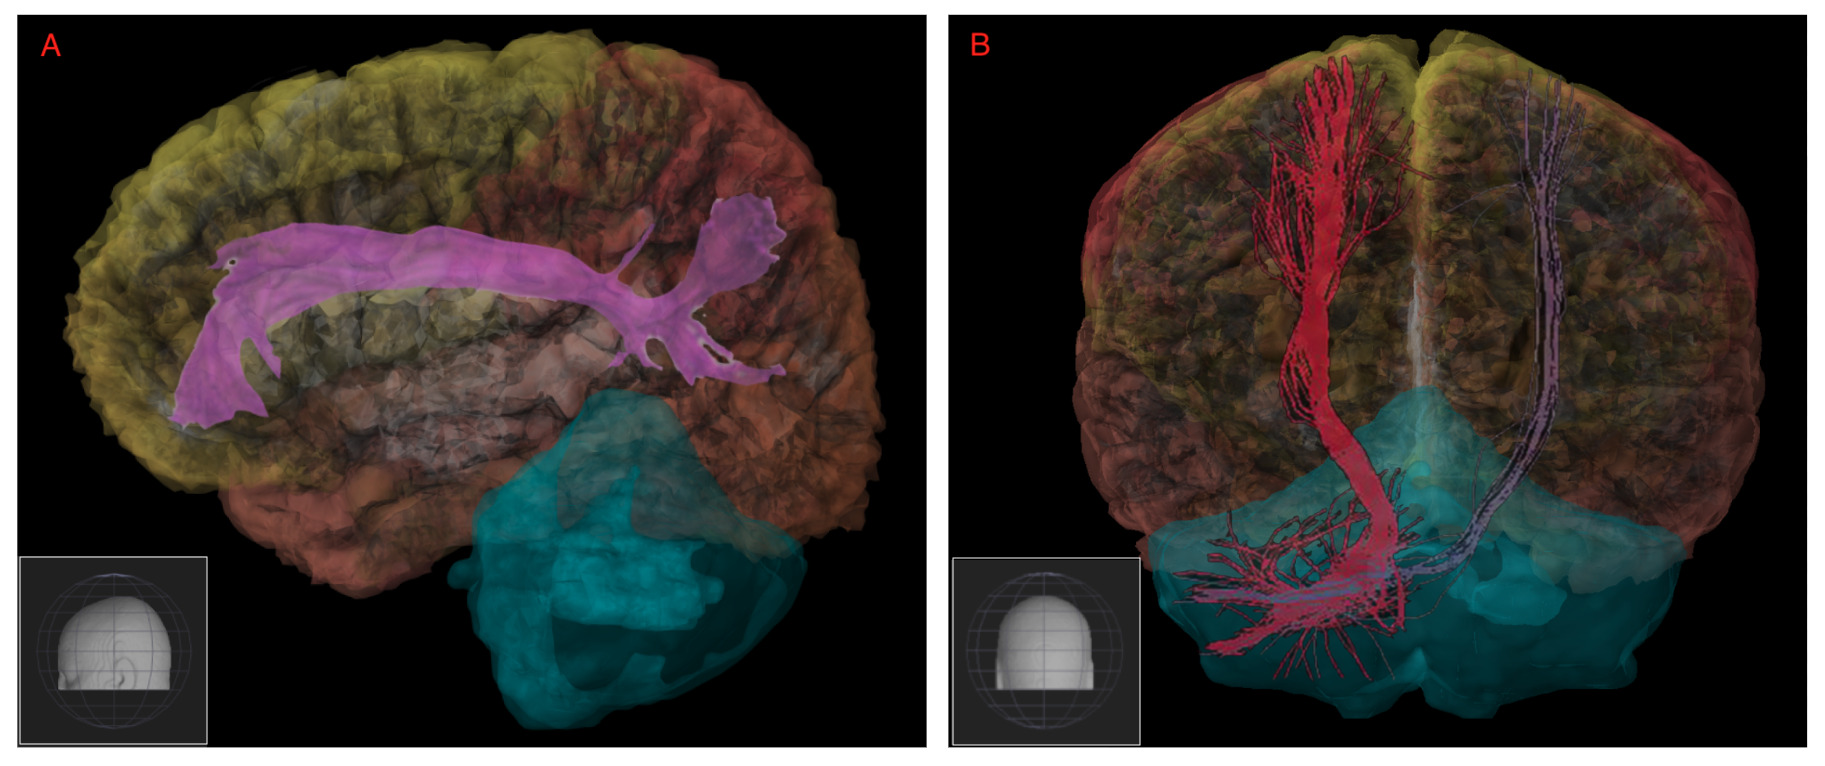
\includegraphics[height=150pt]{./figures/White_Matter_Tracts_Long_Distance.png} %%% 1873 × 810 pixels
  \end{center}
%
  \caption{White matter tracts corresponding to bundles of myelinated neurons speed the transmission of information between distant regions of the brain. The left panel ({\colorred{A}}) shows the connections between the prefrontal cortex and circuits in the parietal and temporal cortex that shape conscious awareness, guide attention and support short-term memory maintenance~\cite{ChicaetalBSF-18,Dehaene2014}. The parietal and temporal cortices are known for being home to {\it{association areas}} that integrate information from multiple sensory systems thereby creating rich representations necessary for abstract thinking. In humans, white matter tracts between the frontal cortex and the cerebellum {\emdash{}} shown in the right panel ({\colorred{B}}) {\emdash{}} facilitate higher-order cognitive function in addition to their role in supporting motor function in all mammals. For example, these connections are particularly important in the development of reading skills in children and adolescents~\cite{TravisetalHBM-15,KozioletalCEREBELLUM-14}.}
%    
  \label{fig_tracts}
%
\end{figure}

%%% %%%%%%%%%%%%%%%%%%%%%%%%%%%%%%%%%%%%%%%%%%%%%%%%%%%%%%%%%%%%%%%%%%%%%%%%%%%%

The cerebellum in mammals serves to shape motor activities selected in the basal ganglia by ensuring they are precisely timed and well-coordinated. Such activities are initiated by the basal ganglia with executive oversight from the prefrontal cortex. In humans, the cerebellum also supports cognitive functions such as those involved in reading~\cite{TravisetalHBM-15}. Figure~{\urlh{#fig_White_Matter_Tracts_Long_Distance}{\ref{fig_tracts}}} ({\colorred{B}}) shows the white matter tracts connecting the cerebellum and prefrontal cortex where such abstract cognitive functions originate. 

A white matter bundle called the {\it{arcuate fasciculus}} {\emdash{}} Figure~{\urlh{#fig_White_Matter_Tracts_Long_Distance}{\ref{fig_tracts}}} ({\colorred{A}}) {\emdash{}} provides reciprocal connections between the frontal cortex and association areas in the parietal and temporal lobes plays a key role in attention and the active maintenance of short-term working memory, including support for language processing in the left hemisphere and visuospatial processing in the right hemisphere~\cite{ChicaetalBSF-18}.

The human brain exhibits structure at many scales, the white matter tracts being but one example. A common pattern involves paths that connect multiple circuits that have their own internal components and connections. At a global scale, processing begins in primary sensory areas, propagates forward through dorsal regions integrating additional sources of information to produce composite representations that are processed in the frontal cortex before returning through ventral regions responsible for motivation and action selection.

%%% %%%%%%%%%%%%%%%%%%%%%%%%%%%%%%%%%%%%%%%%%%%%%%%%%%%%%%%%%%%%%%%%%%%%%%%%%%%%

% RECURRENT FEEDBACK
\subsection{Reciprocity}

%%% %%%%%%%%%%%%%%%%%%%%%%%%%%%%%%%%%%%%%%%%%%%%%%%%%%%%%%%%%%%%%%%%%%%%%%%%%%%%

Many of the connections within such paths are reciprocal allowing feedback to adjust behavior and improve prediction. Similar reflective and self-corrective patterns arise within subcortical regions including the hippocampal complex and basal ganglia, e.g., between the dentate gyrus and CA1 in the hippocampus and as layered networks inside individual subcomponents such as the mossy fiber network within the dentate gyrus. Each level solves different problems, offers general insights and provides hints about how one might realize such solutions in artificial systems.

%%% Advocates of the {\it{two-streams hypothesis}}~\cite{GoodaleandMilnerTiNS-92} contend that sensory processing \emdash{} in particular, seeing and hearing \emdash{} splits into two streams that account for different aspects of perception \emdash{} accounting for {\it{what}} you perceive, e.g., properties of an object, versus {\it{where}} you perceive, e.g., its relative location. 

%%% %%%%%%%%%%%%%%%%%%%%%%%%%%%%%%%%%%%%%%%%%%%%%%%%%%%%%%%%%%%%%%%%%%%%%%%%%%%% 

%%% Figure~{\urlh{#fig_Broadmann_Basal_Ganglia_Hippocampus}{\ref{fig_broadman}}}
\begin{figure}
%
  \begin{center} 
%    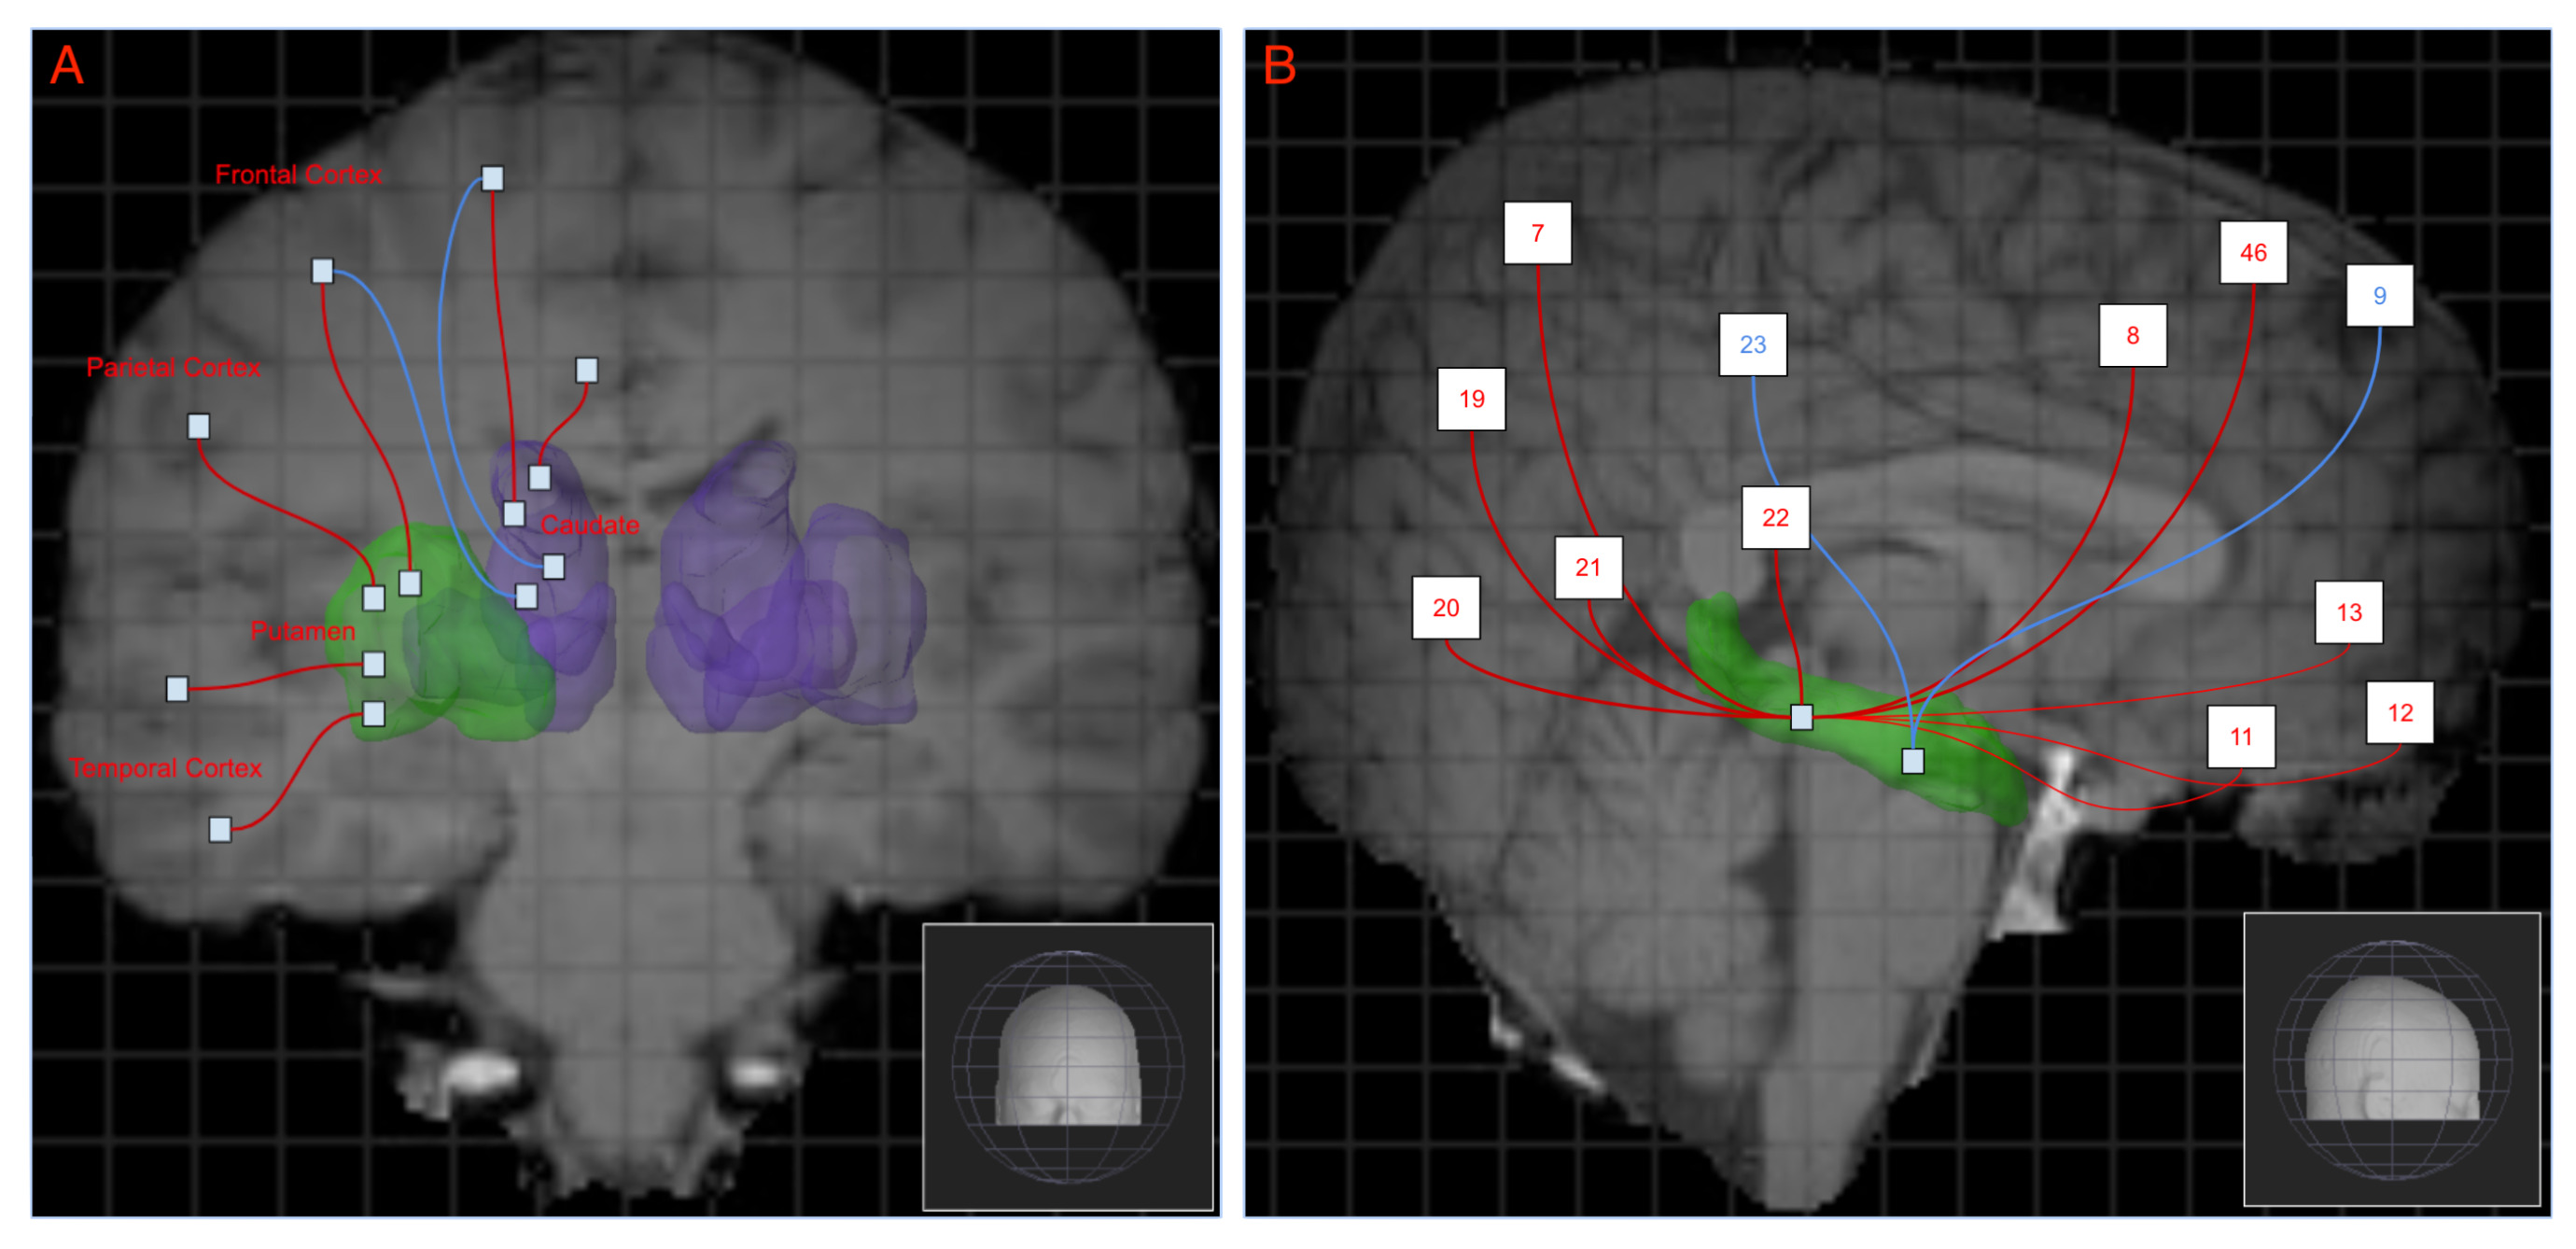
\includegraphics[height=600pt]{./figures/Brodmann_Basal_Ganglia_Hippocampus.png} %%% 2610 × 1290 pixels
    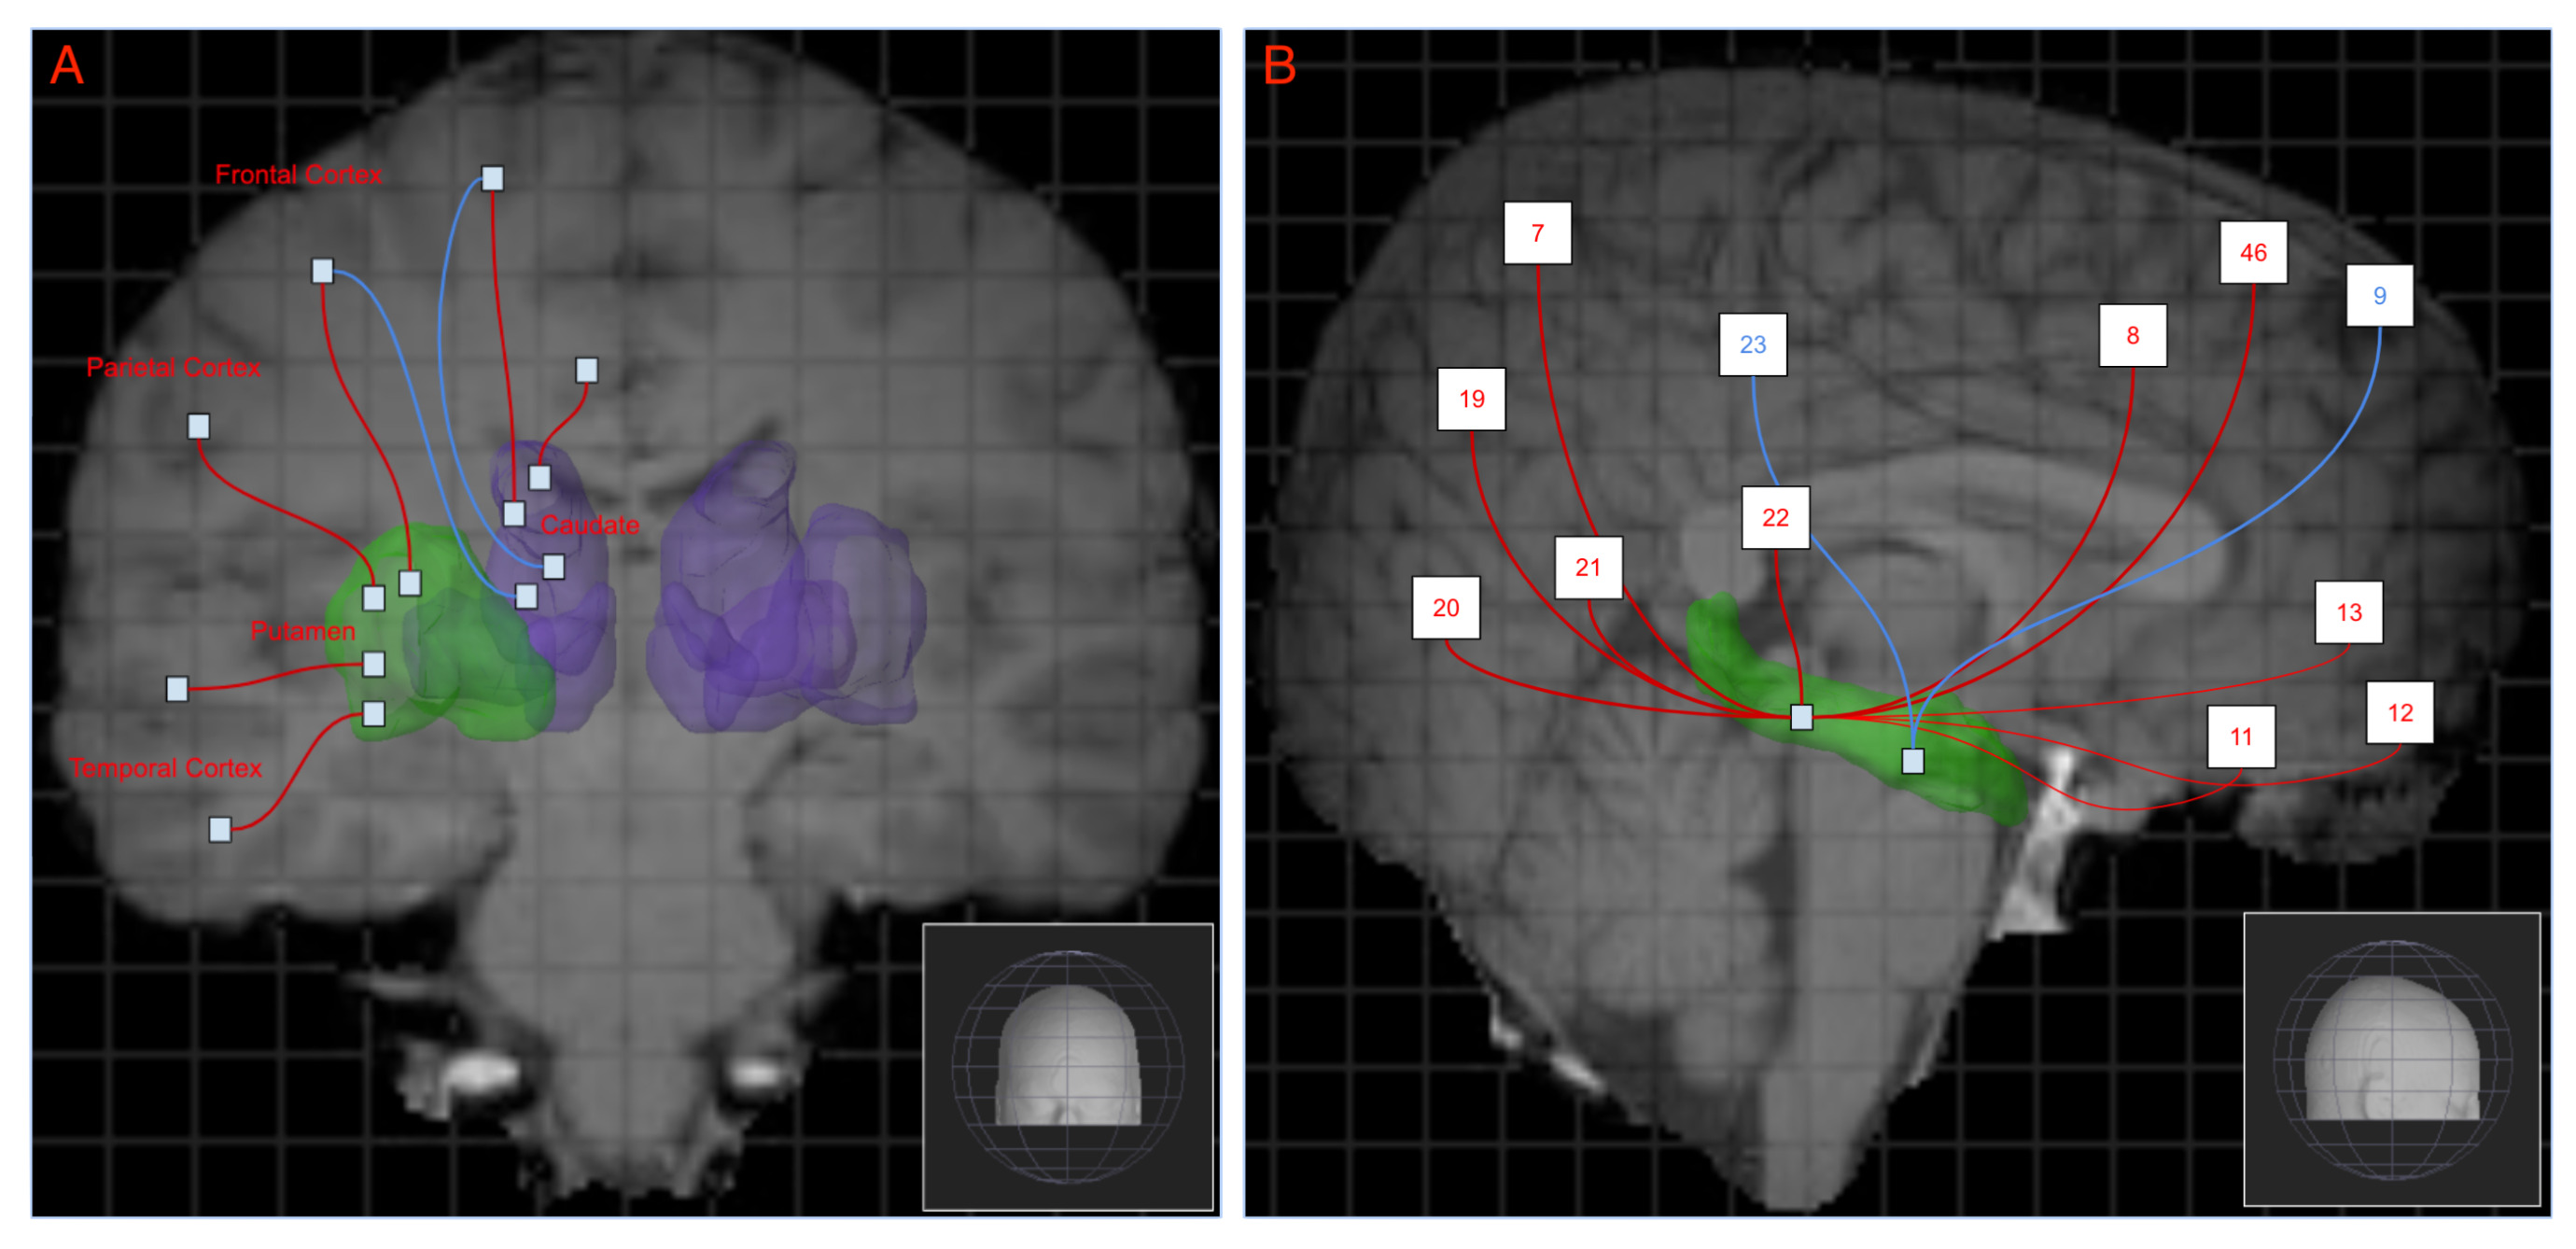
\includegraphics[height=150pt]{./figures/Brodmann_Basal_Ganglia_Hippocampus.png} %%% 2610 × 1290 pixels
  \end{center}
%
  \caption{The left panel ({\colorred{A}}) illustrates the reciprocal connections between two subnuclei of the basal ganglia, the {\it{putamen}} and {\it{caudate nucleus}}, and locations in prefrontal cortex responsible for influencing action selection. The distinctions between frontal, parietal and temporal cortical areas provide only a very general indication of how their function relates to that of the basal ganglia. The right panel ({\colorred{B}}) highlights reciprocal connections between cortical regions {\emdash{}} identified by the Brodmann areas 7, 8, 9, 11, 12, 13, 19, 20, 21, 22, 23 and 46 {\emdash{}} and the hippocampal complex via the adjacent perirhinal (blue) and the parahippocampal (red) areas. The indicated Brodmann areas generally provide a more nuanced understanding of their possible function than does simply stipulating the cortical lobe they reside in.}
%    
  \label{fig_broadman}
%
\end{figure}

%%% %%%%%%%%%%%%%%%%%%%%%%%%%%%%%%%%%%%%%%%%%%%%%%%%%%%%%%%%%%%%%%%%%%%%%%%%%%%%

Figure~{\urlh{#fig_Brodmann_Basal_Ganglia_Hippocampus}{\ref{fig_broadman}}} describes how subcortical nuclei such as the hippocampal complex and basal ganglia interact with cortical regions. Such attributions provide insight on how to construct complex artificial neural architectures composed of simpler subnetworks ostensibly responsible for component functions including perception, action selection and episodic memory.

Here we consider two levels of granularity: the first is coarse grained relying on major anatomical divisions illustrated in Figure~{\urlh{#fig_Human_Brain_Neocortex_Function}{\ref{fig_necortex}}}. The second is somewhat finer grained and relies on areal divisions based on cytoarchitectural distinctions involving cell types, neural processes including dendrites and axons, and other histological characteristics.

The former generally employs Korbinian Brodmann's decomposition of the cortex into 52 {\urlh{https://en.wikipedia.org/wiki/Brodmann_area}{areas}} published in 1909~\cite{Brodmann1909} and revised several times since then to take advantage of more modern staining and imaging technologies as well as improved methods for functional localization. In many cases, identifying the Brodmann area associated with the endpoint of a neural connection can tell us a good deal about the functional relationship between two brain regions.

The left side of Figure~{\urlh{#fig_Brodmann_Basal_Ganglia_Hippocampus}{\ref{fig_broadman}}} ({\colorred{A}}) highlights the reciprocal connections between two subnuclei of the basal ganglia, the {\it{putamen}} and {\it{caudate nucleus}}, and locations in prefrontal cortex responsible for influencing action selection by adjusting input to the basal ganglia and, by way of the thalamus, locations in the parietal and temporal cortex that provide information about the current state relevant to decision making. 

We can often improve functional descriptions if we localize to specific Brodmann areas. For example, the {\it{orbitofrontal cortex}} (OFC) is located in the prefrontal cortex is a region of the frontal lobes involved in the cognitive process of decision-making. In humans it consists of {\it{Brodmann area 10, 11 and 47}}. It is defined as the part of the prefrontal cortex that receives projections from the medial dorsal nucleus of the thalamus, and is thought to represent emotion and reward in decision making~\cite{BotvinickandAnANIPS-09}. The prefrontal cortex, consisting of Brodmann areas 8, 9, 10, 11, 12, 13, 44, 45, 46 and 47, includes the OFC but covers a wider range of functionality.

The right side of Figure~{\urlh{#fig_Brodmann_Basal_Ganglia_Hippocampus}{\ref{fig_broadman}}} ({\colorred{B}}) highlights reciprocal connections between cortical areas {\emdash{}} Brodmann areas 7, 8, 9, 11, 12, 13, 19, 20, 21, 22, 23 and 46 {\emdash{}} and the hippocampal complex via the adjacent {\it{perirhinal}} cortex (shown as blue connections) and the {\it{parahippocampal}} cortex (shown as red connections) that are involved in representing and recognizing objects and environmental scenes.

The anatomy of the brain and patterns of connectivity linking its major functional areas provide a structural account that derives from and informs function. However, functional analyses relating to human cognition require technologies that are able to record neural activity or its correlates aligned with relevant behavioral features. Non-human model systems often employed when invasive technology is required.

On the one hand, optogenetics, two-photon microscopy and conventional electrophysiology are able to record from and modify the electrical activity of tens to thousands of neurons at the resolution of a few microns. While this represents progress, the coverage is inadequate for many studies, and the methods are, for the most part, limited to non-human subjects due to the invasive nature of their practical application~\cite{DombeckandTankCSH-11,BoydenBIOLOGY-11,ZhangetalNATURE-10,YizharetalNEURON-11}.

Conversely, fMRI can used to study awake, behaving humans performing a wide range of cognitive tasks, but relies on signals that are at best indirectly related to neural activity as in the case of blood oxygen levels, and that are currently limited to spatial resolutions on the order of tens of millimeters and temporal resolutions on the order of hundreds of milliseconds~\cite{GoenseetalFiCN-16,GloverPMC-11,BuxtonetalNEUROIMAGING-04}.

Moreover, the electrical activity of individual neurons is but one marker for neural function. Other pathways including diffuse signaling by way of chemical neuromodulation and genetic activity and protein transport at the cellular level are becoming increasingly important as markers for behavior at multiple time scales~\cite{WangandWangFiP-19}. Despite these limitations, neuroscientists have made considerable progress by combining information from different model systems using multiple recording technologies.

%%% %%%%%%%%%%%%%%%%%%%%%%%%%%%%%%%%%%%%%%%%%%%%%%%%%%%%%%%%%%%%%%%%%%%%%%%%%%%%

% SENSORIMOTOR HIERARCHY
\subsection{Sensorimotor Hierarchy}
\label{subsection_sensorimotor_hierarchy}
%%% File: ./inputs/parts/SENSORIMOTOR_HIERARCHY.tex

%%% %%%%%%%%%%%%%%%%%%%%%%%%% BEGIN SENSORIMOTOR HIERARCHY %%%%%%%%%%%%%%%%%%%%%

Much of the cortex is in the business of learning representations of concepts relevant to survival\footnote{%
%
  The word {\it{perspicacity}} refers to a clarity of perception that enables one to recognize subtle differences between similar physical objects or abstract concepts. It is employed in this context to call attention to the fact that attention, exploration, perception, and prediction are inextricably linked in complex biological systems~\cite{RaoandBallardNATURE-NEUROSCIENCE-99,BarlowNC-89,BaddeleyQJoEP-86,ClarkBBS-13}.}.
%
Perception is the means by which we apprehend and act on the physical realization of the concepts we have learned. It seems obvious that perception serves action. It may not seem so obvious that action serves perception, but the fact is we are almost always moving our head, hands and torso in order to resolve ambiguities in what we see, feeling the shape of unfamiliar objects in order to grasp them firmly and twisting about to see who is behind us calling our name or to get a better idea of where we've come from in order to ensure we can retrace our steps. These are complex sensorimotor activities we depend on every day.

In thinking about physically realizable concepts we think first about what they look, feel, sound and smell like. The sensory cortex is responsible for constructing a hierarchy of representations to characterize such concepts, not to capture everything we sense, but rather to account for what we need to know about concepts to survive. Reconstructing scenes with photographic realism is not what our sensory systems were designed for. Circuits of the primary sensory cortex feed into the circuits of the (unimodal) association sensory cortex that feed into (multimodal) sensory cortex. All of these representations are abstract and yet patterns of regionalization are remarkably preserved within species~\cite{ChenetalNEURON-18,PortuguesetalNEURON-14,KolsteretalJoN-09}.

Concepts arise in patterns of neural activity that account for what we need to know about them, including how they appear to us so we can recognize them, what affordances they offer for us to make use of them and how we might predict their occurrence in decision making. Many of the concepts that are represented in our brains serve to model the dynamics of physical systems that we interact with every day, such as riding a bike, working with tools, opening doors, negotiating stairs and riding escalators in department stores. Just as important, if not more so, are the social dynamics we deal with at work and school with their constantly shifting personal relationships and status rankings. 

If you are a software engineer designing robot control systems, you might give action much the same scrutiny as perception and build a parallel hierarchy of representations that describes the concepts that relate to movement including navigation, articulation and manipulation ranging from servo-motor commands to strategies for moving furniture, but designing or learning these hierarchies independently is generally a bad idea. In mammals, these two hierarchies are tightly coupled to account for how they depend on one another~\cite{FusterPREFRONTAL-CORTEX-15}.

Indeed, determining what sensory representations to learn depends upon and influences what motor representations to learn and {\it{vice versa}}, where we follow the convention of using the term {\it{motor}} as a catchall term for concepts relating to muscles and movement. As pointed out in the introduction, there is evidence to suggest that circuits occurring early in the ventral visual stream code for object-selective features and exhibit large-scale organization characterized by the high-level properties of animacy and object size~\cite{KonkleandCaramazzaJoN-13,LongetalPNAS-18}.

%%% %%%%%%%%%%%%%%%%%%%%%%%%%%%%%%%%%%%%%%%%%%%%%%%%%%%%%%%%%%%%%%%%%%%%%%%%%%%%

%%% Figure~{\urlh{#fig_Coupled_Sensory_Motor_Hierarchy}{\ref{fig_coupled}}}
\begin{figure}
%
  \begin{center} 
%     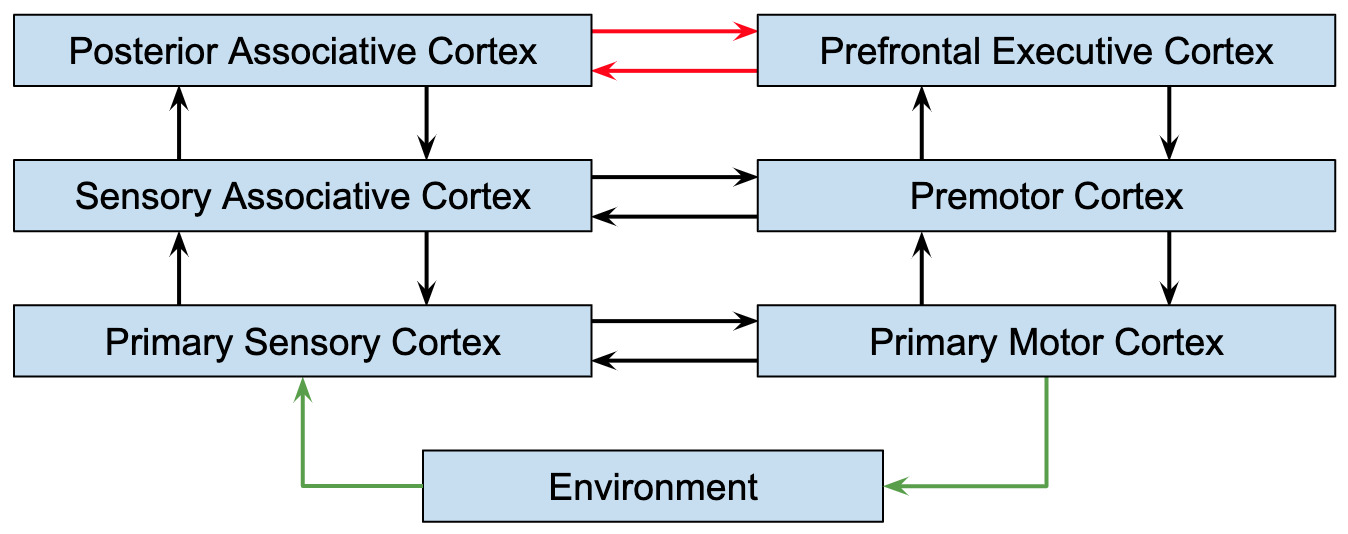
\includegraphics[width=600pt]{./figures/Coupled_Sensory_Motor_Hierarchy.png} %%% 1555 × 635 pixels
    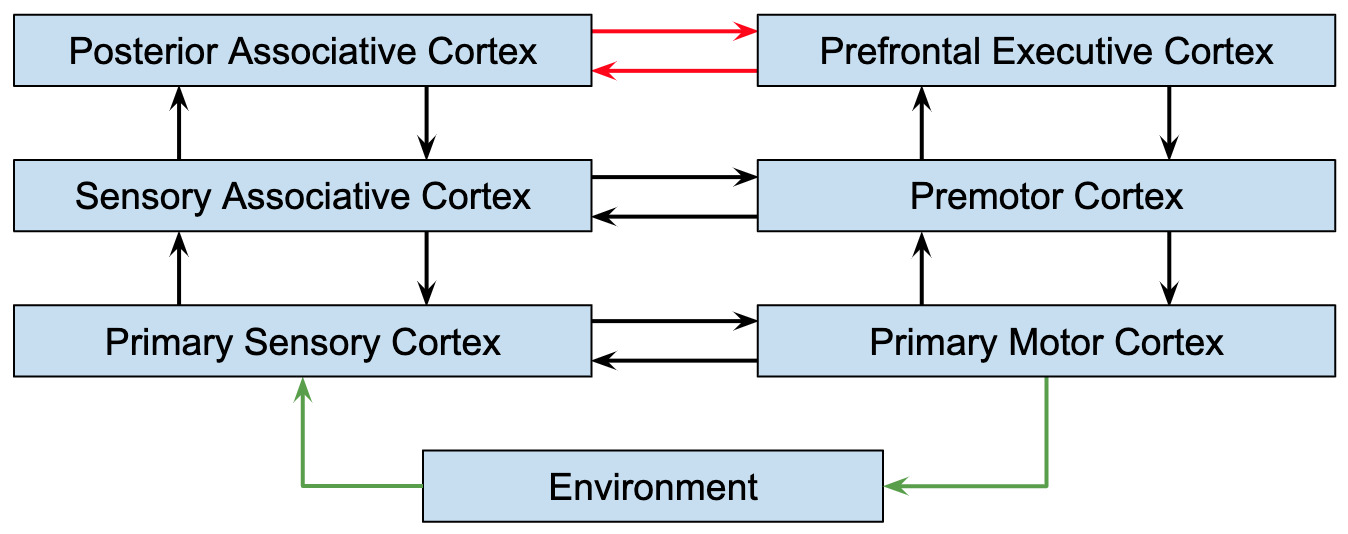
\includegraphics[width=200pt]{./figures/Coupled_Sensory_Motor_Hierarchy.png} %%% 1555 × 635 pixels
  \end{center}
%
  \caption{A simplified block diagram of the cortex. The column on the left represents the posterior cortex including the occipital, temporal and parietal lobes. The column on the right represents the frontal lobe of the cortex corresponding to the primary motor cortex, premotor cortex (association motor cortex) and prefrontal cortex. Green arrows represent interaction with the environment, black arrows represent sensorimotor abstractions and red arrows indicate cognitive activity relating speech, planning and abstract thinking. See the main text for more detail. Adapted from Figure~8.9 in~\cite{FusterPREFRONTAL-CORTEX-15-CHAPTER_8}}
%    
  \label{fig_coupled}
%
\end{figure}

%%% %%%%%%%%%%%%%%%%%%%%%%%%%%%%%%%%%%%%%%%%%%%%%%%%%%%%%%%%%%%%%%%%%%%%%%%%%%%%

Figure~{\urlh{#fig_Coupled_Sensory_Motor_Hierarchy}{\ref{fig_coupled}}} is a simplified block diagram of the cortex organized as two columns. The left column represents the posterior cortex consisting of the occipital, temporal and parietal lobes that are primarily concerned with processing sensory information. The relevant brain areas are summarized in three blocks roughly corresponding to primary sensory cortex, unimodal association cortex and multimodal association cortex stacked so the least abstract concepts are on the bottom and most abstract on the top. The combined area is often referred to as {\it{semantic memory}} and characterized as long-term declarative memory~\cite{BinderandDesaiTiCS-11}. 

The right column represents the frontal lobe of the cortex corresponding to the primary motor cortex, premotor cortex (associative motor cortex) and prefrontal cortex. The primary motor cortex is responsible for creating abstract representations of motor activity throughout the body. The premotor cortex is responsible for integrating sensory and motor abstractions to construct sensorimotor representations. The prefrontal cortex orchestrates cognitive behavior including speech, planning and abstract thinking, and is reciprocally connected to the association areas just mentioned as well subcortical structures including the basal ganglia and hippocampus.

The two columns are connected with one another at multiple levels: by physical interaction with the environment (green arrows), by sensorimotor abstraction and alignment (black arrows), and by cognitive effort in directing activity mediated through subcortical structures (red arrows). This arrangement supports the formation of rich representations that serve a wide range of cognitive function. The sensorimotor connections and feedback through the environment provide an inductive bias to guide learning, ground inference and reduce sample complexity by reducing reliance on labeled data and enabling opportunities for unsupervised learning~\cite{BarlowNC-89}.

Simple as this model of cortical function may seem, it may be one of the most important architectural contributions of neuroscience to the development of artificial intelligence patterned after the human brain. Some of the lessons have already been integrated into the discipline of control theory through exposure to early work in biological cybernetics~\cite{FukushimaBC-80,Lettvinetal59,Jackson1958selected,GibsonPERCEPTION-50,McCullochandPitts43,vonUexk1926theoretical}, but some of the most important lessons impact the application of machine learning in building autonomous embodied systems including robots and digital assistants as alluded to above. 

%%% %%%%%%%%%%%%%%%%%%%%%%%%%% END SENSORIMOTOR HIERARCHY %%%%%%%%%%%%%%%%%%%%%%


%%% %%%%%%%%%%%%%%%%%%%%%%%%%%%%%%%%%%%%%%%%%%%%%%%%%%%%%%%%%%%%%%%%%%%%%%%%%%%%

% ACTION SELECTION
\subsection{Basal Ganglia}
\label{subsection_basal_ganlia}
%%% File: /inputs/parts/BASAL_GANGLIA_MOTOR.tex

%%% %%%%%%%%%%%%%%%%%%%%%%%%%%%%%%%%% BEGIN BASAL GANGLIA %%%%%%%%%%%%%%%%%%%%%%%%%%

There is a long history of neuroscientists constructing computational models of human cognition~\cite{McClelland79,McClellandandRumelhartPR-88,LebiereandAndersonCSS-93,OReillySCIENCE-06,BotvinickPTRS_B-07}. Different modeling tools make different assumptions and support different levels of detail from rule-based systems to spiking neurons~\cite{OReillyetalLEABRA-16,OReillyetalCCN-12,RasmussenetalPLoS-ONE-17,Eliasmith2013,BlouwandEliasmithCSS-13,JilketalJETAI-08}. In this paper, we are primarily concerned with computational models that leverage ideas from neuroscience to develop AI systems for practical problems. In this subsection and the next, we take a closer look at the basal ganglia and hippocampus using models from neuroscience that reveal computational principles we can apply in a wide range of practical problems.

%%% In this section, we consider the biological basis for action selection and higher order executive control in human beings. In particular we looks at the neural circuits generally considered to be our best guess about how reinforcement learning in implemented in the brain. These circuits assist in formulating and carrying out plans to achieve our goals and solving complex problems that require a high degree of attention, the capacity to hold several concepts in mind at a time and the ability to think about how these concepts relate to one another so as to draw new conclusions. 

%%% In each case, we start with a simplified introduction to the relevant anatomy, followed by an explanation of how the biological networks support the target capability. Later, we provide an example artificial neural network that supports a related, if not precisely equivalent capability. The two capabilities that we consider are also noteworthy for the fact that each relies upon subcortical regions that every mammal comes equipped with.  However, these functional areas have evolved considerably in humans over the last few million years as they have adapted to take advantage of and support the extended capabilities of the mammalian human neocortex.

In contrast with the relative simplicity of the neocortical architecture, the {\it{basal ganglia}} consist of specialized subcortical nuclei that are related by their evolved function. In the following, we emphasize and simplify some of those nuclei and ignore others to focus the discussion and simplify the biology. The basal ganglia provide the basis for motor activity controlled by circuits in the brainstem and conserved throughout vertebrate evolution for nearly half a billion years. The cerebral cortex has been around in the form of a six-layer sheet tiled with a repeating columnar structure since the early mammals came on the scene in the Jurassic period about 200 million years ago. Our lineage separated from mice around 100 million and from macaques and other old world monkeys around 25 million years ago. The modern human neocortex owes much to these earlier evolutionary innovations but is different in ways that make possible our facility with language, complex social organization and sophisticated abstract thinking. Compared with the basal ganglia, the neocortex is structurally elegant and functionally general.

The basal ganglia have evolved along with our neocortex to provide us with a powerful thinking machine, while at the same time leaving us to make do with some less-than-ideal adaptations. We can simulate a conventional computer in our heads but are limited to fewer than a dozen memory registers. Most of us can't perform long division in our heads even though we might know the algorithm and aided with paper and pencil carry out the necessary computations to produce an answer. We rely on the same basic cognitive machinery we use to list a few names in alphabetical order to perform all sorts of more complicated cognitive tasks. Even simpler, however, is the basic operation of choosing one of several actions to perform next. The basal ganglia play a key role in supporting action selection and it is worth looking at in a little more detail in order get a handle on some of the parts of the brain that figure prominently in human cognition. Recall that the cortex is a sheet of neural tissue more or less homogeneous in terms of its local structure quite unlike almost any other part of the brain except for the cerebellar cortex. The cortex sits on top of a structure called the {\it{thalamus}} which among other things serves as a relay in passing information back and forth between the cortex and various subcortical nuclei.

The basal ganglia consist of a bunch of circuits, of varied size, sometimes but not always consisting primarily of one cell type, sometimes but not necessarily compactly clustered together, sporting projections that seem to wander off aimlessly, but more or less located above the brainstem and below the cortex. As a general principle, if a signal sets off along some path exiting from a circuit, then expect some derivative of that signal to appear later reentering the circuit to serve as feedback. Everything about the brain, and your entire body for that matter, has to be carefully regulated to maintain a dynamic state of equilibrium, and unlike human designs, evolution is generally not able to cleanly separate the parts of the circuit that perform computations in service to behavior from those that deal with respiration, immune response, waste removal, cell repair, death and regeneration, etc. 

%%% %%%%%%%%%%%%%%%%%%%%%%%%%%%%%%%%%%%%%%%%%%%%%%%%%%%%%%%%%%%%%%%%%%%%%%%%%%%%

%%% Figure~{\urlh{#fig_Basal_Ganglia_Anatomy_and_Physiology}{\ref{fig_basal}}}
\begin{figure}
%
  \begin{center}
%    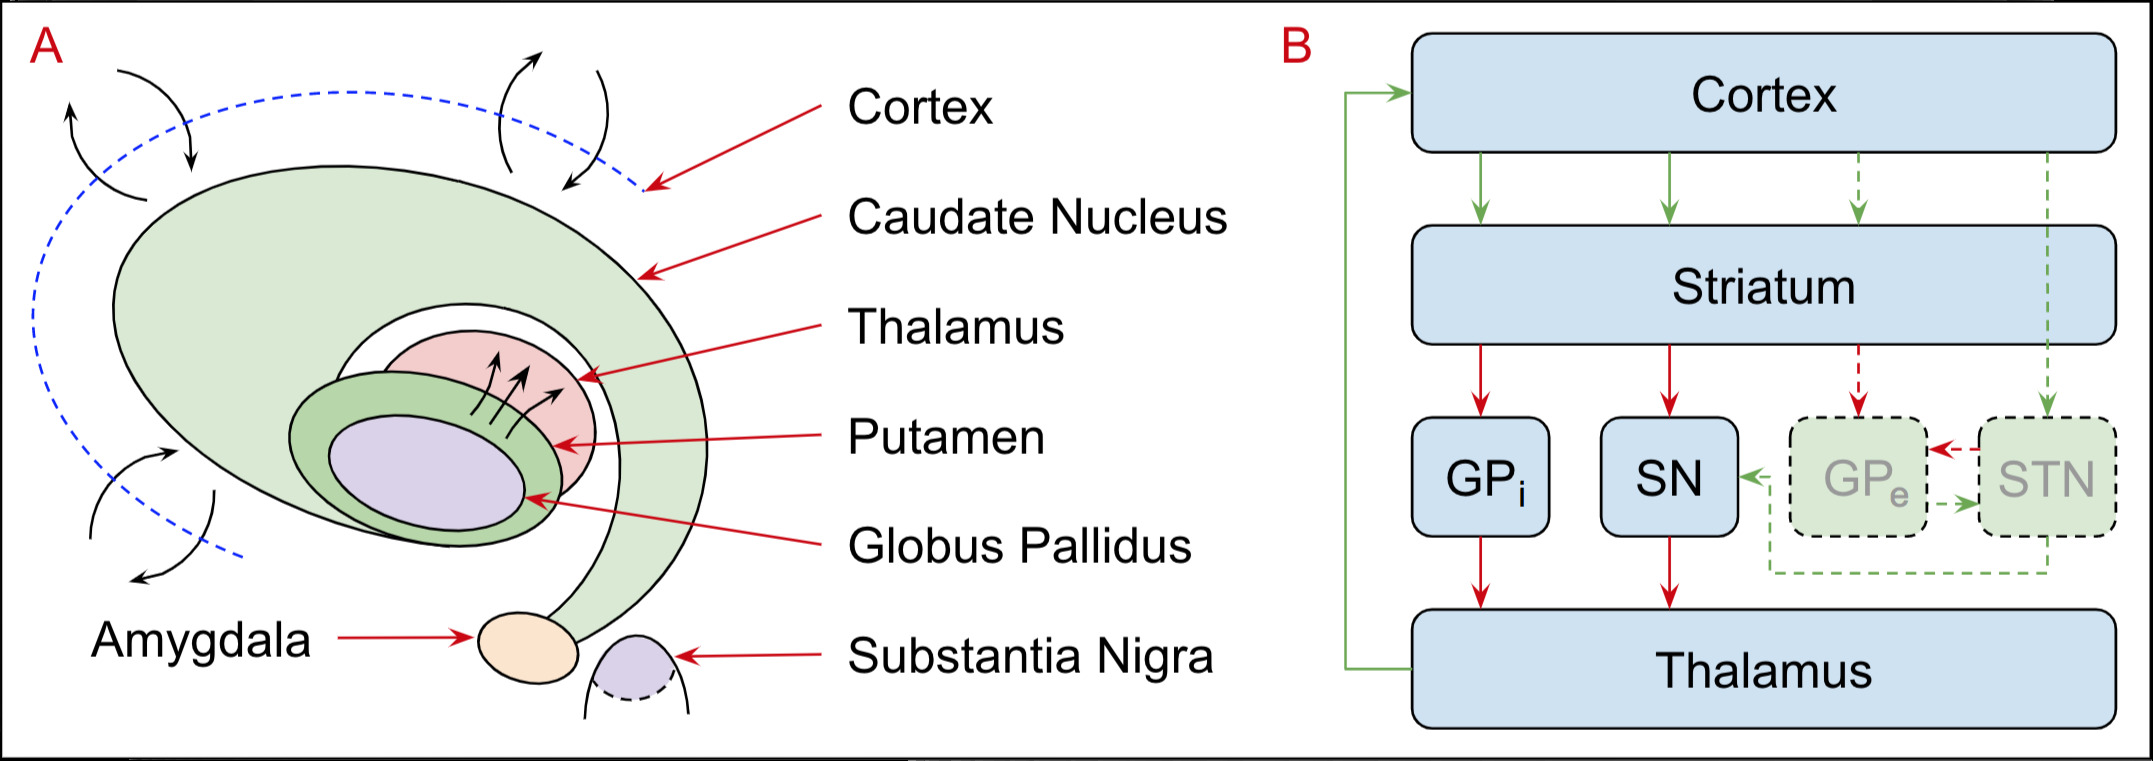
\includegraphics[width=9.0in]{./figures/Basal_Ganglia_Anatomy_and_Physiology.png} %%% 2194 × 803 pixels @ 72 per inch
    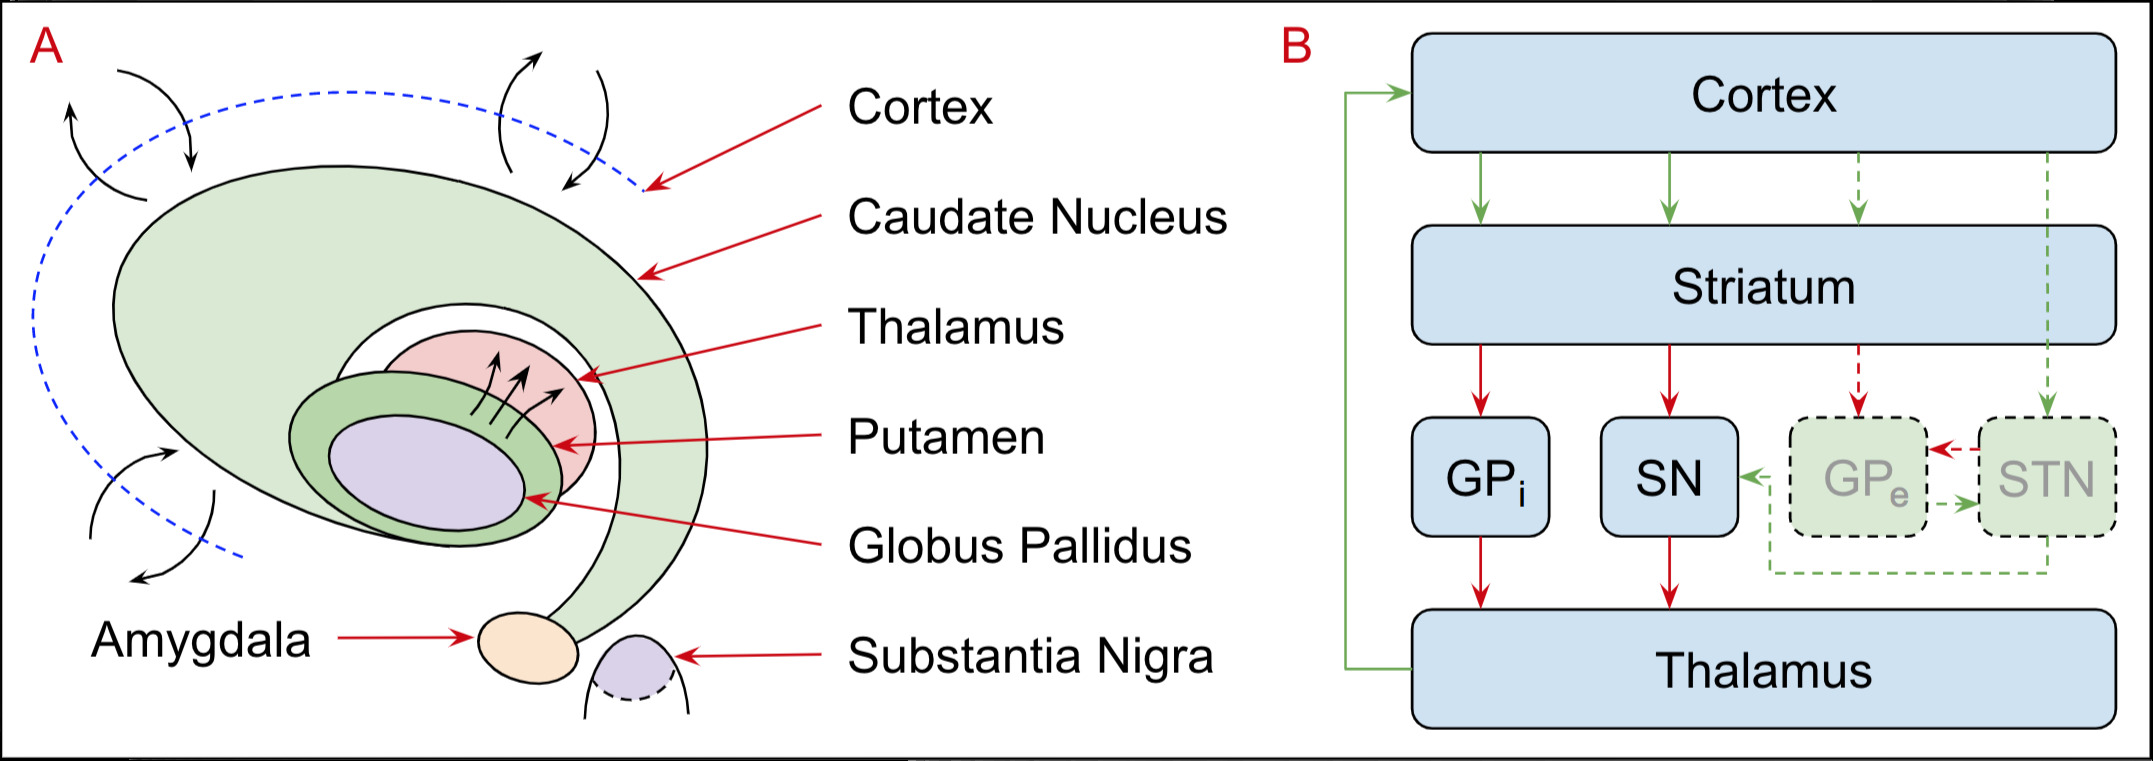
\includegraphics[width=4.0in]{./figures/Basal_Ganglia_Anatomy_and_Physiology.png} %%% 2194 × 803 pixels @ 72 per inch
  \end{center}
%
  \caption{The left panel ({\colorred{A}}) provides a highly stylized anatomical drawing of the basal ganglia. Figure~\ref{fig_broadman} ({\colorred{A}}) provides more anatomical detail while the above drawing abstracts from the structural detail in order to simplify the functional account. The block diagram shown in the right panel ({\colorred{B}}) depicts the primary components involved in action selection as functional blocks. The blocks shown in blue represent components in the {\it{direct path}} and are described in the text proper. The blocks shown in light green with dashed borders represent additional components that contribute to the {\it{indirect path}}. Good explanations of the indirect path are described in O'Reilly~\etal{}~\cite{OReillyetalCCN-12} or Wang~\etal{}~\cite{WangetalNATURE-NEUROSCIENCE-18} and we return to the basal ganglia in the next section when we look at the executive role of the prefrontal cortex in modulating behavior.}
%
  \label{fig_basal}
%
\end{figure}

%%% %%%%%%%%%%%%%%%%%%%%%%%%%%%%%%%%%%%%%%%%%%%%%%%%%%%%%%%%%%%%%%%%%%%%%%%%%%%%

The basal ganglia are depicted in Figure~{\urlh{#fig_Basal_Ganglia_Anatomy_and_Physiology}{\ref{fig_basal}}} ({\colorred{A}}) taking some artistic license to keep things simple. The thalamus along with another structure called the {\it{striatum}} provide the interface between the cortex and basal ganglia. The striatum is a combination of a number of smaller nuclei that are anatomically and functionally related; they include the Globus Pallidus (GP), Putamen and Caudate Nucleus and aside from their function as part of the striatum, only the GP will figure prominently in our discussion and only one part of it \emdash{} referred to as the {\it{internal}} GP and identified with the "i" subscript to distinguish it from the {\it{external}} part with "e" subscript.

The other players include the Substantia Nigra (SN) which is at one end of the striatum nestled close to the {\it{amygdala}} which is part of the limbic system involved with memory, decision-making and modulating emotional responses, and the Subthalamic Nucleus (STN). You can think of the cortex as integrating sensory and motor information and making suggestions for what action to take next and the amygdala as supplying information pertaining to the possible emotional consequences of taking different actions to be used as input to action selection. Figure~{\urlh{#fig_Basal_Ganglia_Anatomy_and_Physiology}{\ref{fig_basal}}} ({\colorred{B}}) reconfigures these component nuclei into a smaller number of functionally motivated blocks that control two pathways \emdash{} the {\it{direct pathway}} associated primarily with inhibition and consisting of the internal GP and SN and the {\it{indirect pathway}} playing an excitatory role and consisting of the external GP and STN~\cite{OReillyetalCCN-12,WangetalNATURE-NEUROSCIENCE-18},

The lines connecting the functional blocks shown in Figure~{\urlh{#fig_Basal_Ganglia_Anatomy_and_Physiology}{\ref{fig_basal}}} ({\colorred{B}}) imply neural connectivity, with arrows indicating the direction of influence and colors indicating the valence of the influence, green for excitatory and red for inhibitory. In the action selection cycle, the cortex forwards activations that you can think of as suggestions for what action to take next. These suggestions are propagated through the striatum and forwarded along the direct pathway where two stages of inhibitory neurons initially suppress all of the suggestions and propagate signals back the cortex to activate inhibitory neurons that suppress activity at the source. As this cycle continues, an additional process takes place in the indirect path \emdash{} identified with dashed lines \emdash{} that weighs the advantages and disadvantages of the proposed actions taking in information from throughout the cortex and adjusting the inhibitory bias accordingly.

Eventually, one proposal wins out and all of the others are suppressed allowing a single preferred action to be executed. This cycle of exploring the options for acting and then selecting a single action to execute is constantly repeated during your waking hours. Additional machinery in the thalamus and brain stem regulate whether or not to forward suggestions for acting during sleep when your cortex receives no sensory input and hence any suggestions for acting uninformed by sensory input are ill-advised if not outright dangerous. The above description doesn't begin to convey the complexity of what's going on at the level of individual neurons. Suffice it to say that the usual perfunctory summary consisting of "the winner takes all" doesn't begin to do it justice. The subtleties that arise from the way in which the evidence for and against an action proposal is combined, how ties are broken and deciding when enough evaluation is determined sufficient to make a final choice. 

%%% %%%%%%%%%%%%%%%%%%%%%%%%%%%%%%%%%% END BASAL GANGLIA %%%%%%%%%%%%%%%%%%%%%%%%%%%


%%% %%%%%%%%%%%%%%%%%%%%%%%%%%%%%%%%%%%%%%%%%%%%%%%%%%%%%%%%%%%%%%%%%%%%%%%%%%%%

% MEMORY SYSTEMS
\subsection{Hippocampal Complex}
\label{subsection_hippocampus}
%%% File: ./inputs/parts/HIPPOCAMPAL_COMPLEX.tex

%%% %%%%%%%%%%%%%%%%%%%%%%%%%%%%%% BEGIN HIPPOCAMPAL COMPLEX %%%%%%%%%%%%%%%%%%%%%%%

Figure~{\urlh{#fig_Hippocampus_Anatomy_and_Physiology}{\ref{fig_hippo}}} provides a glimpse of how we construct memories of our experience and subsequently retrieve those memories to support a diverse range of cognitive strategies. In this case, the {\it{hippocampus}} will play a central role as did the basal ganglia in the previous example. In the next section, we explore how the basal ganglia work in concert with the hippocampus to support reinforcement learning. For now, our goal is simply to describe the process whereby we consolidate and then encode experience. In doing so we take the opportunity to talk about the process whereby we retrieve memories, reconstruct a version of that past experience to perform counterfactual inference and imagine possibilities that we have never actually experienced. 

%%% %%%%%%%%%%%%%%%%%%%%%%%%%%%%%%%%%%%%%%%%%%%%%%%%%%%%%%%%%%%%%%%%%%%%%%%%%%%%

%%% Figure~{\urlh{#fig_Hippocampus_Anatomy_and_Physiology}{\ref{fig_hippo}}}
\begin{figure}
%
  \begin{center}
%    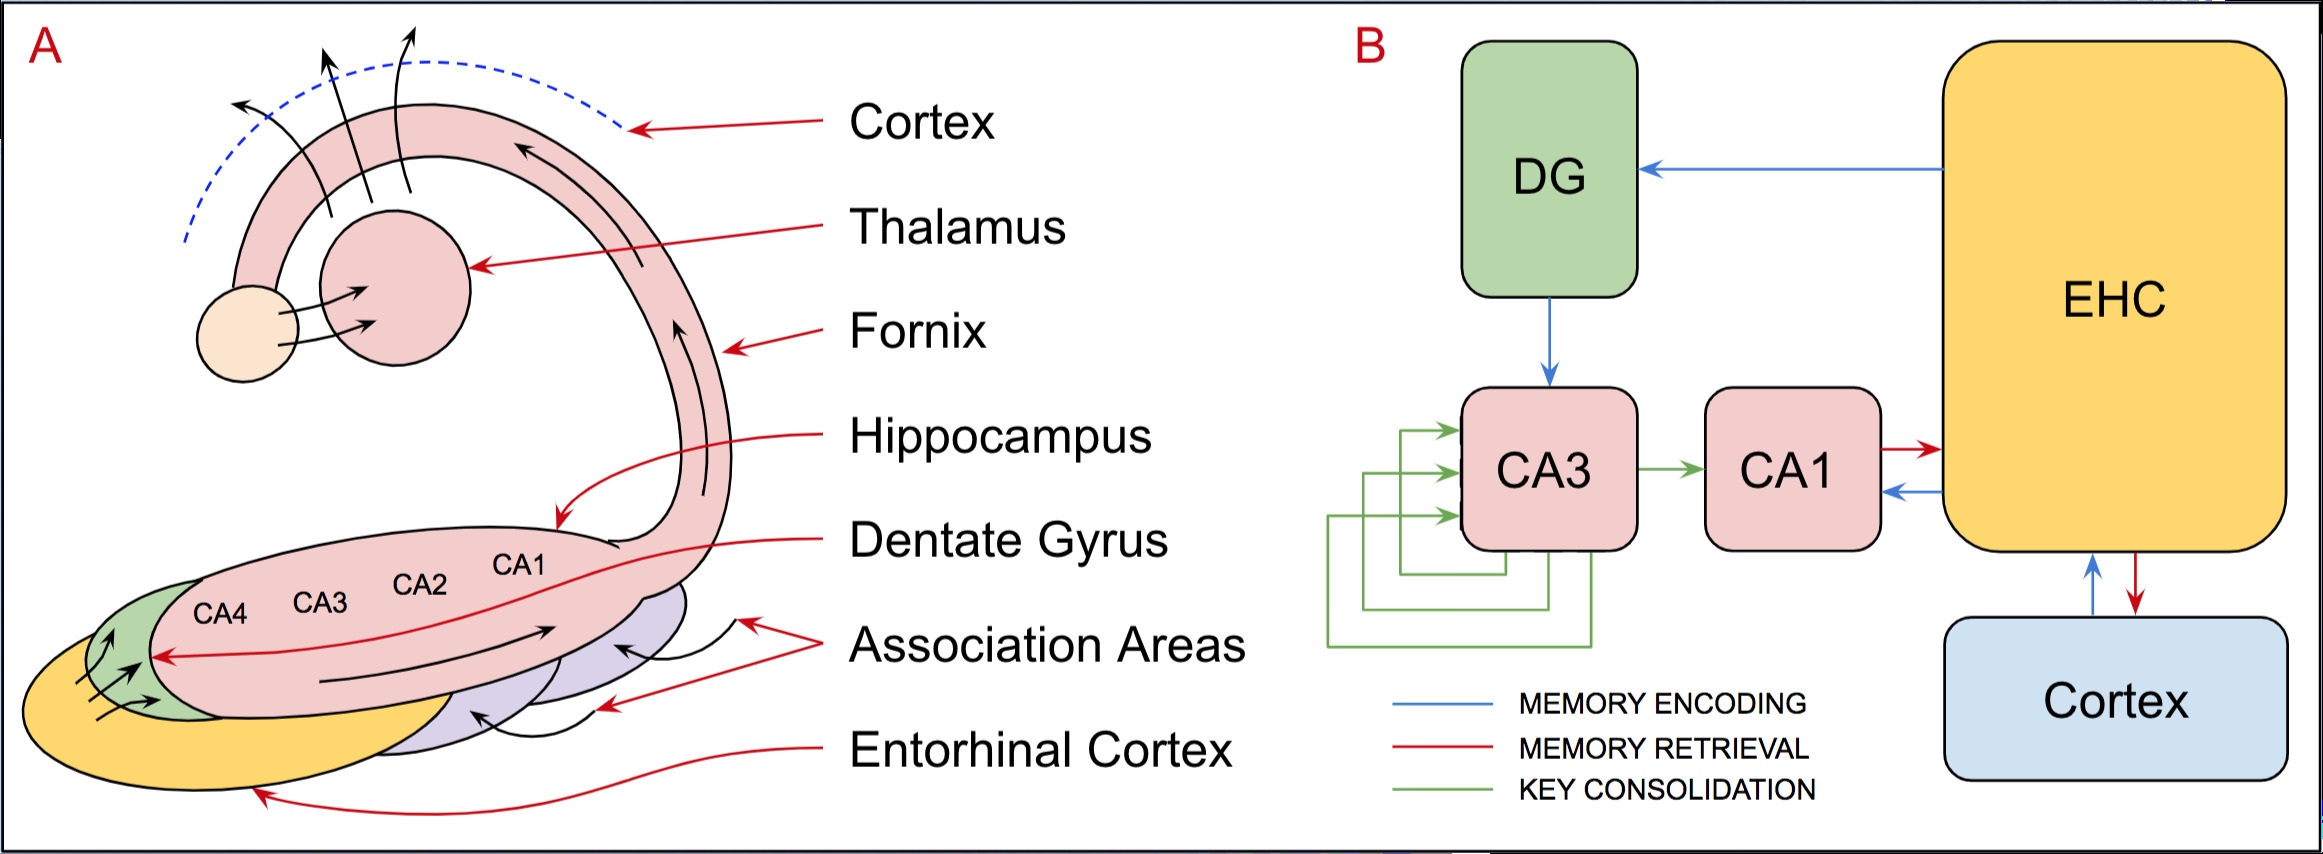
\includegraphics[width=10.0in]{./figures/Hippocampus_Anatomy_and_Physiology.png} %%% 2362 × 900 pixels @ 72 per inch
    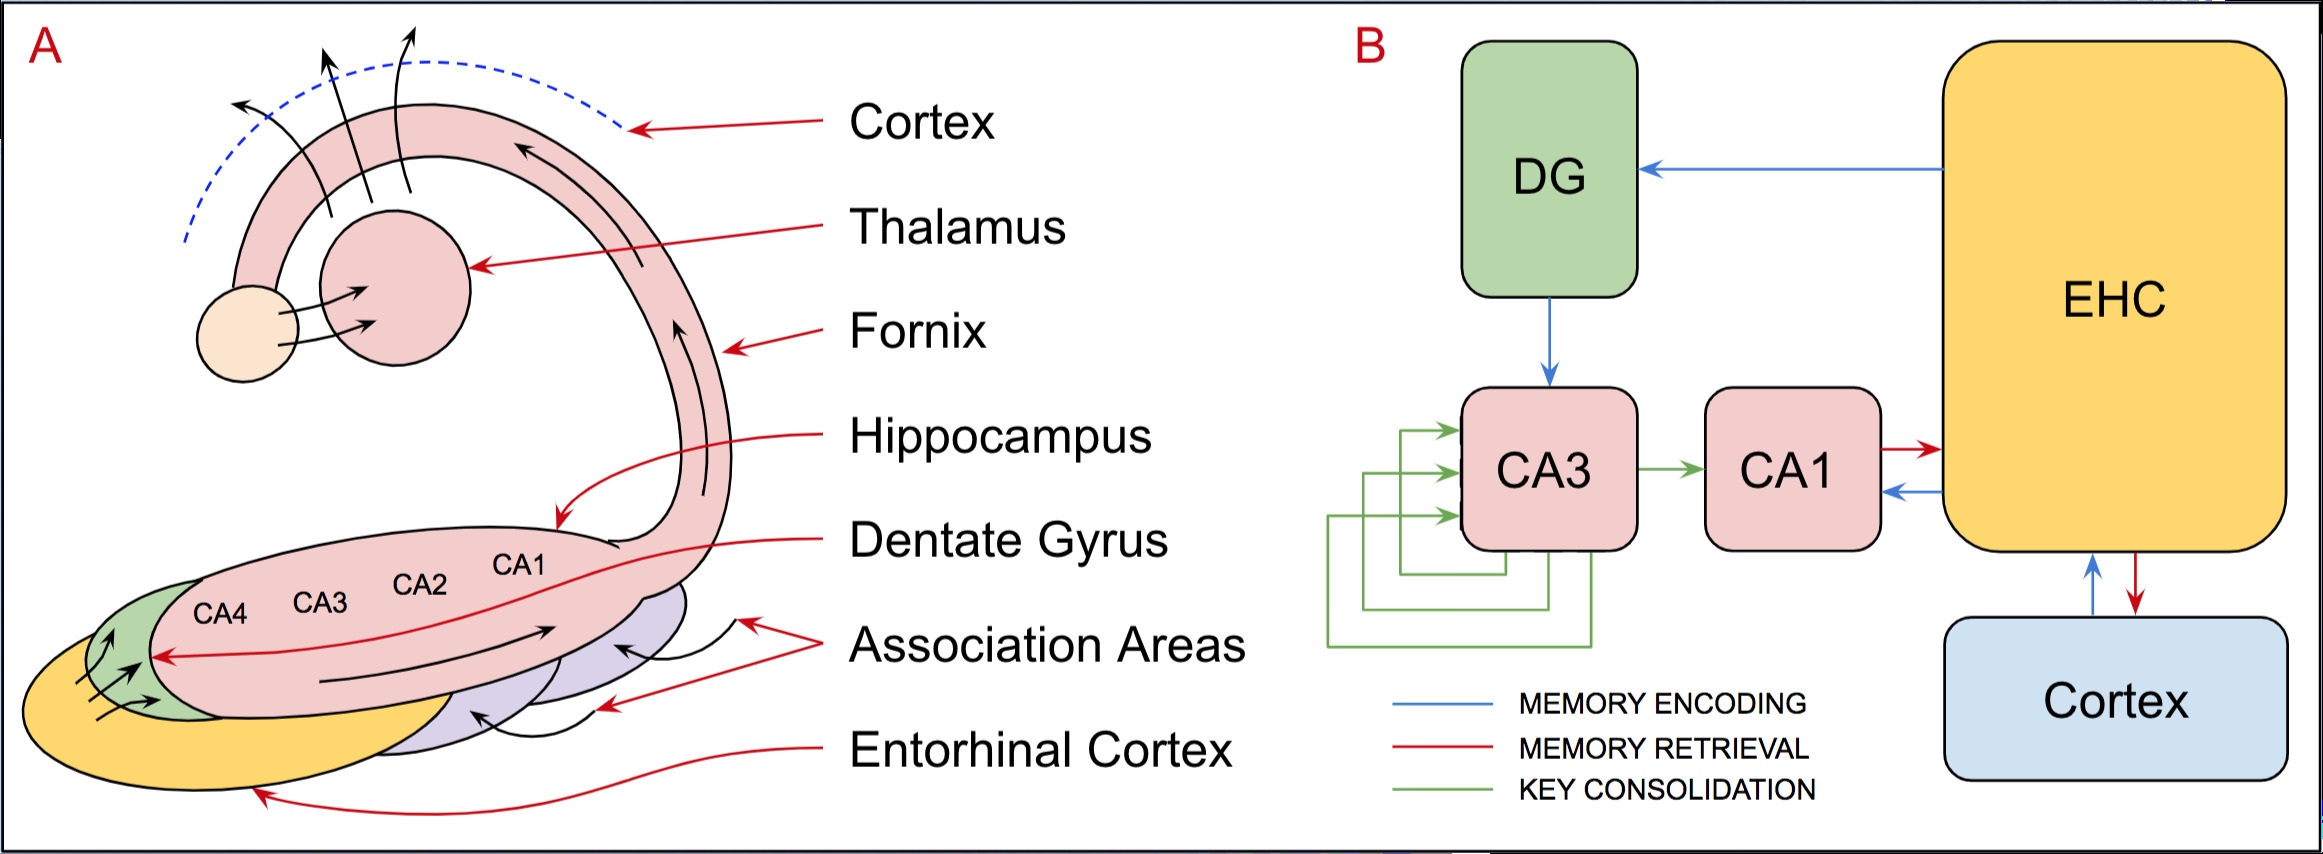
\includegraphics[width=4.0in]{./figures/Hippocampus_Anatomy_and_Physiology.png} %%% 2362 × 900 pixels @ 72 per inch
  \end{center}
%
  \caption{On the left you see a cartoon drawing of the hippocampus and related cortical and subcortical areas. The primary components include the entorhinal cortex or EHC, the dentate gyrus or DG and two hippocampal (out of four) nuclei referred to as CA3 and CA1. Figure~\ref{fig_broadman} provides additional anatomical detail regarding the connections between cortical regions and the perirhinal and parahippocampal areas adjacent to the hippocampus. The block diagram on the right summarizes the component circuits, along with their projections and reciprocal connections.}
%
  \label{fig_hippo}
%
\end{figure}

%%% %%%%%%%%%%%%%%%%%%%%%%%%%%%%%%%%%%%%%%%%%%%%%%%%%%%%%%%%%%%%%%%%%%%%%%%%%%%%

The name {\it{hippocampus}} like so many biological terms has obscure origins, generally in Latin or Greek and in this case the latter, relating to its shape that looked like a seahorse to some early anatomists. As shown in Figure~{\urlh{#fig_Hippocampus_Anatomy_and_Physiology}{\ref{fig_hippo}}} ({\colorred{A}}) it is primarily comprised of four subnuclei referred to as CA1, CA2, CA3 and CA4, the first two characters in each abbreviation recalling a previous Latin name, {\it{Cornu Ammanonis}} associated with a ram's horn, apparently preferred by even earlier anatomists. These nuclei are capped by the {\it{dentate gyrus}} (DG) at one end and the {\it{fornix}} at the other\footnote{%
%
  The hippocampus plays an important role in the transfer of information from short-term memory to long-term memory during encoding and retrieval stages. These stages need not occur successively, but are broadly divided in the neuronal mechanisms they require or even in the hippocampal areas they activate. According to Michael Gazzaniga, "encoding is the processing of incoming information that creates memory traces to be stored." There are two steps to encoding: acquisition and consolidation. During acquisition, stimuli are committed to short term memory. Consolidation is where the hippocampus along with other cortical structures stabilize an object within long term memory. ({\urlh{https://en.wikipedia.org/wiki/Hippocampal_memory_encoding_and_retrieval}{SOURCE}})}. 

The hippocampus consists of two nearly identical structures, one in each hemisphere, connected where the parallel tracts of the fornix come together at the midline of the brain. The hippocampus is tightly coupled with the {\it{entorhinal cortex}} (EHC) that plays an important role in memory, navigation and our perception of time. Information flows from the EHC to the hippocampus by one of two pathways: either through the DG to CA3 or via reciprocal connections to and from CA1. The EHC also has reciprocal connections to many cortical areas. Figure~{\urlh{#fig_Brodmann_Basal_Ganglia_Hippocampus}{\ref{fig_broadman}}} ({\colorred{A}}) provides additional anatomical detail. 

In the process of creating a new memory, the hippocampus receives input from multiple cortical areas relevant to current experience, consolidates this information in a condensed format that will enable subsequent retrieval and stores the resulting encoding in memory. In retrieving an existing memory, The EHC starts with cortical activity, typically from motor and sensory association areas, and uses this information to reconstruct a previous memory by activating cortical areas corresponding to the original memory. Before describing how we think such creative consolidation and subsequent reconstruction works, a word about why this process is beneficial might be in order.

Almost every stage of memory is fraught with opportunities to alter stored representations of prior experience. Reconstruction is a creative process in which we are more often than not forced to fill in some details that we might think we observed at the time but actually didn't. In the formation of new memories, consolidation can only make do with whatever information about the experience we have gleaned from observation and committed to short-term memory. If you don't rehearse what you've stored in short-term memory then it will quickly fade, losing detail and potentially introducing errors of omission and commission.

%%% You might purposely or unconsciously alter what you think you remember to conveniently leave the impression that you behaved different than you actually did. There are all kinds of reasons to alter your memories to suit your purposes just as there all sorts of reasons for lying to ourselves~\cite{Trivers2011}. Self-deception can offer interpersonal benefits that offset its costs in whatever currency you value most. There is evidence to suggest that people lie to convince themselves of the truth of their persuasive goal, and by doing so, are able to argue their case more persuasively to others~\cite{SmithetalJEP-17}. 

%%% This sort of imaginative reconstruction has called into question the accuracy of first-person accounts and expert witnesses. But it also explains our eminently useful commonsense application of believable counterfactual reasoning, e.g., if I hadn't had that second cup of coffee, I would have slept better last night~\cite{ParikhetalNEUROIMAGE-18,DeBrigardetalNEUROIMAGE-15}. And, considered in the context of avoiding dangerous situations, planning for contingencies, or imagining a world very different from the one in which we live, one that can inspire and motivate us to act to achieve such a future, it underscores the amazing strength, resilience and determination of the human mind.

The basic algorithm carried out by the hippocampus and entorhinal cortex working together is illustrated in Figure~{\urlh{#fig_Hippocampus_Anatomy_and_Physiology}{\ref{fig_hippo}}} ({\colorred{B}}). There are two basic processes that we consider here: encoding new memories and retrieving old memories. Encoding involves collecting information gleaned from diverse neural activity originating in multiple cortical regions and consolidating~\cite{MorrisetalNEURON-06} this information to construct a compact encoding that serves as a key or index that will enable subsequent stable \emdash{} meaning reliably consistent even in the presence of distracting information~\cite{EisenbergetalSCIENCE-03} \emdash{} retrieval and reconstruction\footnote{% 
%
   Memory consolidation is a category of processes that stabilize a memory trace after its initial acquisition. Consolidation is distinguished into two specific processes, synaptic consolidation, which is synonymous with late-phase long-term potentiation and occurs within the first few hours after learning, and systems consolidation, where hippocampus-dependent memories become independent of the hippocampus over a period of weeks to years. Recently, a third process has become the focus of research, reconsolidation, in which previously-consolidated memories can be made labile again through reactivation of the memory trace. ({\urlh{https://en.wikipedia.org/wiki/Memory_consolidation}{SOURCE}})}.

EHC receives input from all cortical regions in a condensed form and the axons of EHC pyramidal neurons project primarily to the DG but also to CA1. DG then projects to CA3 which plays a particularly important role in encoding and retrieving memories. CA3 is thought to behave as an autoassociative memory shown here as a recursive neural network. The crucial property of an autoassociative memory is that it is able to retrieve an item from memory using only a portion of the information associated with that item\footnote{%
% 
  {\it{Autoassociative memories}} are capable of retrieving a piece of data upon presentation of only partial information. {\it{Hopfield networks}} are recurrent artificial neural networks that have been shown to act as an autoassociative memory since they are capable of remembering data by observing a portion of that data. Hopfield networks can be trained with a variety of different learning methods including Hebbian learning which is often summarized as "neurons that fire together wire together". ({\urlh{https://en.wikipedia.org/wiki/Hopfield_network}{SOURCE}})}. 

%%% For example, this property allows us to retrieve information about a party that was held years ago just by catching a glimpse of a person on the street who happens to look like someone whom we first met at that party. You can think of your observation of the person from the party as a probe or key that enables you to access and unlock that earlier experience. Of course, you could have simply mistaken that person you saw on the street for the person you met at the party.

%%% Hippocampal indexing theory~\cite{TeylerandDiScennaBEHAVIORAL-NEUROSCIENCE-86} hypothesizes that when we have a conscious experience, different areas of the cortex are activated related to that experience such as activity in the auditory cortex resulting from our listening to a recording of Yo-Yo Ma playing Bach or activity in the visual cortex produced by a particularly vivid sunset we witnessing. When we remember the experience later, similar areas of the cortex are reactivated allowing us to re-experience the event.

The hippocampus serves as an index, storing different patterns of cortical activity and allowing us to retrieve our memories using only a fragment of what we can recall. The recurrent connections of CA3 are thought to enable this sort of creative reconstruction and play a role in both encoding and retrieving memories. CA3 then projects to CA1 and from there back to the EHC completing the loop and thereby providing recurrent activity involving a much larger circuit.

%%% %%%%%%%%%%%%%%%%%%%%%%%%%%%%%%%%%%%%%%%%%%%%%%%%%%%%%%%%%%%%%%%%%%%%%%%%%%%%

There are a couple of details that are worth pointing out here as they demonstrate both the strengths and weaknesses of human episodic memory. The first concerns the issue of retrieving a complete memory given a partial index and the second concerns how to retrieve a memory when that memory is similar to one or more other memories, at least in the sense that their respective indices are similar to one another. In the model described here, the first issue is handled by the autoassociative network.

%%% %%%%%%%%%%%%%%%%%%%%%%%%%%%%%%%%%%%%%%%%%%%%%%%%%%%%%%%%%%%%%%%%%%%%%%%%%%%%

%%% Figure~{\urlh{#fig_Hippocampus_Auto_Associative_Network}{\ref{fig_assoc}}}
\begin{figure}
%
  \begin{center}
%    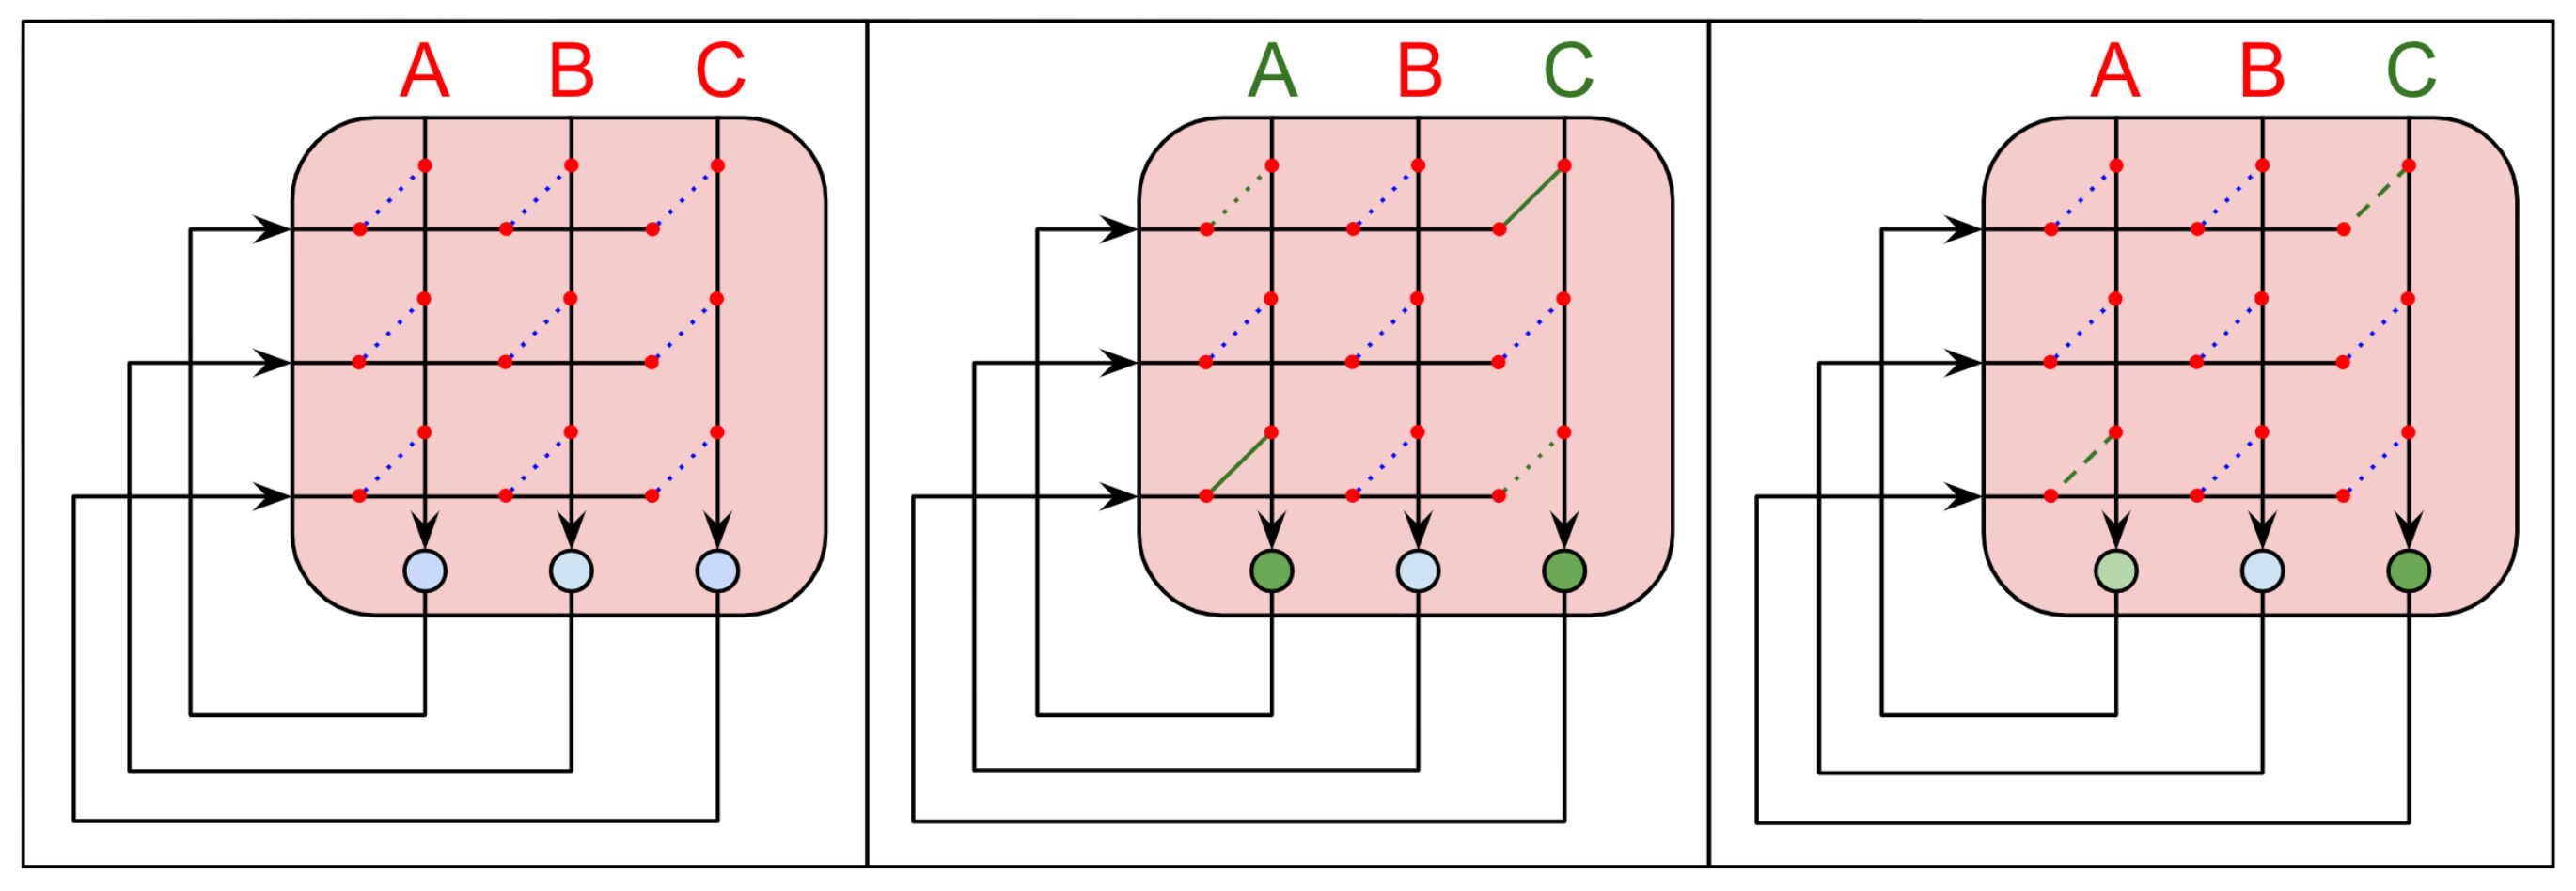
\includegraphics[width=7.5in]{./figures/Hippocampus_Auto_Associative_Network.png} %%% 2540 × 887 pixels
    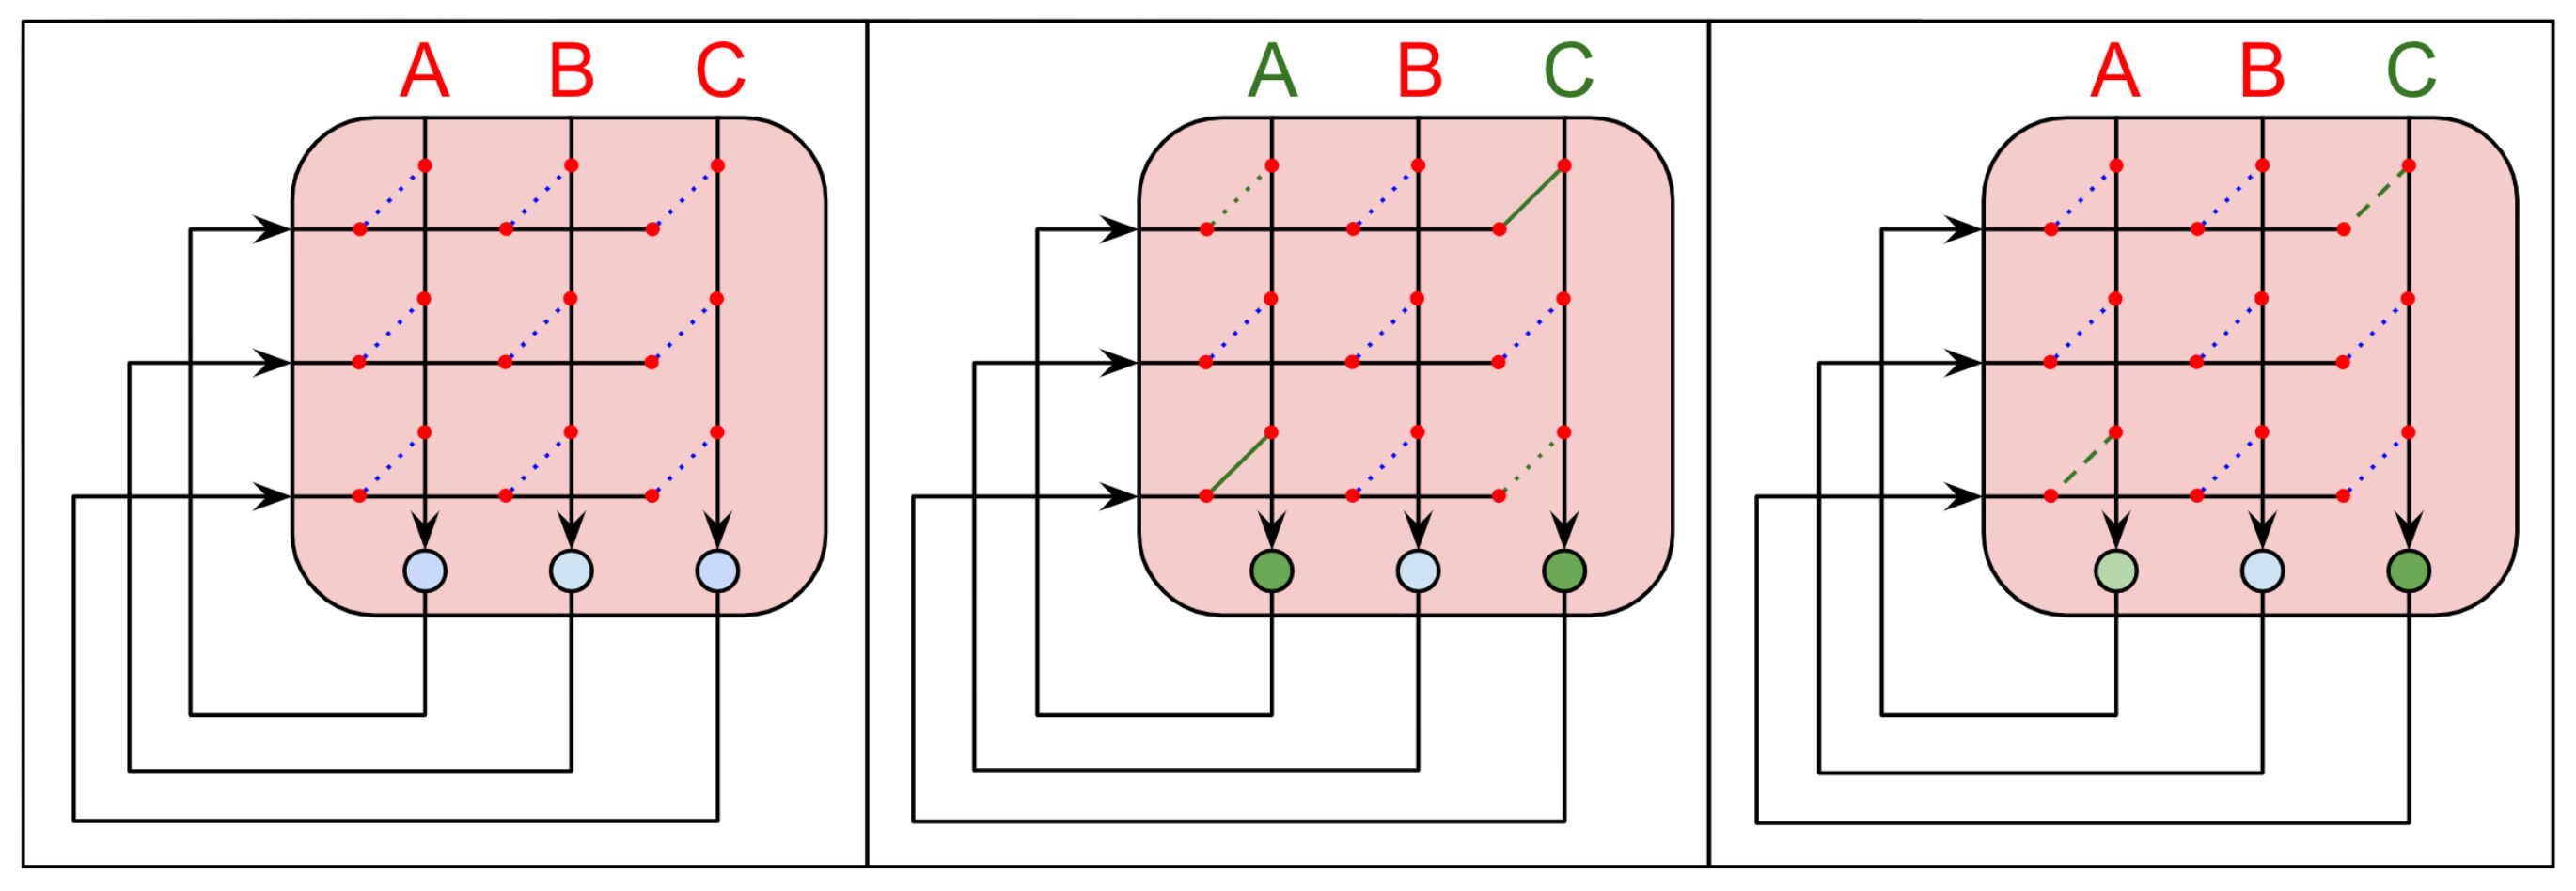
\includegraphics[width=3.25in]{./figures/Hippocampus_Auto_Associative_Network.png} %%% 2540 × 887 pixels
  \end{center}
%
  \caption{The three panels shown here represent the autoassociative network representing the function of CA3 in the hippocampus. Connection weights are shown as diagonal lines, e.g., the dotted blue lines shown in the network on the far left represent the connection weights prior to any training. The middle panel represents the network after encoding the stimulus pattern corresponding to the cortical activation of A and C, and the panel on the far right represents the network, when presented with a partial pattern consisting of just C, employing the recurrent connections of the autoassociator to complete the pattern for the original stimulus and using it to reconstruct the corresponding activation of A and C in the cortex.}
%
  \label{fig_assoc}
%
\end{figure}

%%% %%%%%%%%%%%%%%%%%%%%%%%%%%%%%%%%%%%%%%%%%%%%%%%%%%%%%%%%%%%%%%%%%%%%%%%%%%%%

The triptych shown in Figure~{\urlh{#fig_Hippocampus_Auto_Associative_Network}{\ref{fig_assoc}}} illustrates how the autoassociative network solves this problem. The panel on the far left is meant to indicate the autoassociative network and its initial state. In the middle panel, we assume the input from the dentate gyrus consist of the two sub patterns A and C and illustrates the reciprocal connections that would be strengthened were we to train the network with this composite pattern of activity. CA3 is responsible for encoding these memory specific patterns of activity for all of our memories.  The panel on the far right is intended to illustrate how given a partial pattern, in this case just one of the two representative patterns that comprise the composite pattern shown in the middle panel, is able to reconstruct the other representative pattern by using the trained autoassociative network to first identify and then strengthen the connections in the original composite.

The second detail concerns the possibility that the encodings for two memories are alike enough to be mistaken with one another. A full account of any of the theories explaining how the human brain solves this problem is beyond the scope of what we can go into here but one theory \emdash{} first articulated by David Marr~\cite{MarrandBrindleyPTRS_B-71,WillshawetalPTRS_B-15} \emdash{} posits that, since the dentate gyrus has a larger number of cells than the EHC, its forward projection will tend to produces an expansion recoding in the DG leading to an increase in the separation between the patterns in CA3. %%% Evidence from recordings in mice and computational modeling using artificial neural network and dynamical system models offer support for the theory~\cite{NeunuebelandKnierimNEURON-14}. 

%%% %%%%%%%%%%%%%%%%%%%%%%%%%%%%%%%%%%%%%%%%%%%%%%%%%%%%%%%%%%%%%%%%%%%%%%%%%%%%

%%% Memory consists of patterns of cortical activations which can be condensed and
%%% sent to the entorhinal cortex, undergo pattern separation and then bound together
%%% are indexed in the CA3 auto associator.  

%%% Then when a feature of the original stimulus is present it activates a subpopulation
%%% of the original neurons activated in the CA3 and the recurrent connections reactivate
%%% the remaining neurons making up the pattern,

To complete our account of memory retrieval, we look at how the path that started in the EHC loops back to complete a feedback loop that stabilizes the encoding of memories. So far we've seen how an experience represented by a pattern of activity in the cortex is compressed and represented in the entorhinal cortex which projects this pattern onto the cells in the dentate gyrus thereby increasing the separation between competing patterns the results of which are bound together to generate an index. This index is fed to CA3 where it is incorporated in an autoassociative recursive network so that subsequently when a feature of the original stimulus is present in our conscious experience it activates a subset of the original neurons activated in CA3 and the recurrent connections in the autoassociative network reactivate the remaining neurons completing the pattern that was incorporated when the experience was initially encoded in memory.
  
%%% The final step is to see how the reactivates the original stimulus. This is thought
%%% to be mediated by CA1. The entorhinal cortex not only projects to the dentate gyrus,
%%% it also projects to CA1.

%%% This means that when the neurons are activated in CA3, also activated in CA1 is
%%% another representation of the cortical path. Since these populations of neurons are
%%% activated at the same time, they undergo long-term potentiation and the connections
%%% between them are strengthened.

%%% The above account provides a clear unique role for every area in the system, except
%%% for area CA1 - what is the unique role of CA1? In the original CLS work,
%%% including McClelland and Goddard (1997), we theorized that CA1 is critical for
%%% developing a sparse, invertible mapping. This means that activity patterns produced
%%% by incoming cortical activity during encoding are capable of re-creating those same
%%% cortical activity patterns during retrieval without which, catastrophic interference
%%% would remain, regardless of how effective the pattern separation is within the CA3.

The remaining step involves explaining how the representation in CA3 reactivates the original stimulus. As shown in Figure~{\urlh{#fig_Hippocampus_Anatomy_and_Physiology}{\ref{fig_hippo}}} ({\colorred{B}}), the entorhinal cortex projects to CA1 in addition to the dentate gyrus. When neurons are projected forward to DG and activated in CA3 they are also activated in CA. Since they are activated at the same time, the connections between the neurons in CA3 and CA1 are strengthened by long-term potentiation\footnote{%
%
  In neuroscience, long-term potentiation (LTP) is a persistent strengthening of synapses based on recent patterns of activity. These are patterns of synaptic activity that produce a long-lasting increase in signal transmission between two neurons. The opposite of LTP is long-term depression, which produces a long-lasting decrease in synaptic strength. It is one of several phenomena underlying synaptic plasticity, the ability of chemical synapses to change their strength. As memories are thought to be encoded by modification of synaptic strength, LTP is widely considered one of the major cellular mechanisms that underlies learning and memory. ({\urlh{https://en.wikipedia.org/wiki/Long-term_potentiation}{SOURCE}})}.
%
The result is a stable, sparse, invertible mapping that allows the hippocampus to recreate the original cortical activity patterns during retrieval~\cite{OReillyetalCS-15,McClellandandGoddardHIPPOCAMPUS-97}. Reactivating the same combination of cortical areas as the original stimulus and causing us to reexperience the event as a memory. An additional process called {\it{reconsolidation}} is thought to allow previously-consolidated memories become labile again as a consequence of reactivation\footnote{%
%
  Memory reconsolidation is the process of previously consolidated memories being recalled and actively consolidated. It is a distinct process that serves to maintain, strengthen and modify memories that are already stored in the long-term memory. Once memories undergo the process of consolidation and become part of long-term memory, they are thought of as stable. However, the retrieval of a memory trace can cause another labile phase that then requires an active process to make the memory stable after retrieval is complete. It is believed that post-retrieval stabilization is different and distinct from consolidation, despite its overlap in function. ({\urlh{https://en.wikipedia.org/wiki/Memory_consolidation}{SOURCE}})}.
%
See {\urlh{box_patterns}{Box~\colorred{A}}} for detail on storing and retrieving memories in the hippocampus.

%%% %%%%%%%%%%%%%%%%%%%%%%%%%%%%%%%%%%%%%%%%%%%%%%%%%%%%%%%%%%%%%%%%%%%%%%%%%%%%
   
%%% This means that neurons in CA3 activate the neurons in CA1 corresponding to the
%%% correct cortical areas. These then project back to the entorhinal cortex which
%%% has reciprocal connections to many areas of the cortex. Reactivating the same
%%% combination of cortical areas as the input and causing us to reexperience the
%%% event as a memory.

%%% %%%%%%%%%%%%%%%%%%%%%%%%%%%%%%% END HIPPOCAMPAL COMPLEX %%%%%%%%%%%%%%%%%%%%%%%%


%%% %%%%%%%%%%%%%%%%%%%%%%%%%%%%%%%%%%%%%%%%%%%%%%%%%%%%%%%%%%%%%%%%%%%%%%%%%%%%

%%% File: ./inputs/boxes/BOX_CHAOFEI_FAN.tex

\begin{center}
  %%% \begin{tcolorbox}[sharp corners=all,coltitle=black,colbacktitle=white,
  \begin{tcolorbox}[breakable,sharp corners=all,coltitle=black,colbacktitle=white,
    width=\textwidth,boxsep=5pt,left=5pt,right=5pt,
    title={\textbf{Box A: Pattern Separation, Completion and Integration}}]

    %%% width=\textwidth,boxsep=5pt,left=5pt,right=5pt,hypertarget={box_patterns},

    %%% Pattern separation is defined as the process by which overlapping or similar inputs
    %%% (representations) are transformed into less similar outputs [...] pattern completion
    %%% is defined as the reconstruction of complete stored representations from partial 
    %%% inputs that are part of the stored representation (Colgin et al., 2008; Wilson, 2009). 

~~~~{\it{Pattern separation}} reduces the similarity between input patterns of activity by orthogonalizing inputs to minimize interference between patterns and increase hippocampal storage capacity~\cite{KesnerandRollsNBR-15}. Pattern separation involves primarily dentate gyrus (DG) and hippocampal CA3. The DG maps input from entorhinal cortex (EHC) to a much larger and sparsely active granule cells (GCs) population. In rats, the number of neurons in the DG exceeds that in EHC by about 5:1~\cite{DrewetalLEARNING-MEMORY-13}. This expansion coding with strong inhibitory interneurons and a competitive learning rule can greatly reduce the overlap between inputs. The DG connects to CA3 mainly through {\it{mossy fibers}} that reliably activate CA3 pyramidal neurons and sustain activation for tens of seconds~\cite{VyletaetalELIFE-16}. Each CA3 neuron receives a small number of these connections from DG so the degree of sparsity is maintained~\cite{KesnerandRollsNBR-15}.

~~~~{\it{Pattern completion}} reconstructs the complete stored pattern given a partial input. Each pyramidal neuron in CA3 receives a large number of synapses from other pyramidal cells forming a recurrent network that serves as an autoassociative memory for pattern completion~\cite{KesnerandRollsNBR-15}. During learning, recurrent connections between active CA3 neurons are strengthened and later when neurons encoding part of an episode are reactivated, they recurrently activate other connected cells to reconstruct the original episode. Basket cells in CA3 form inhibitory synapses to pyramidal cells to dampen excitatory responses thereby emphasizing key features~\cite{NeunuebelandKnierimNEURON-14}. 

~~~~Pattern completion provides access to relevant experience to support decision making in novel situations, and while pattern separation helps downstream discrimination, perfectly orthogonal representations are not ideal in the case we want events that occurred close together to have similar representations. In this case, {\it{pattern integration}} represents related experiences as overlapping populations. There are a number of neural mechanisms suggested to support pattern integration in the hippocampus. We consider two here, the first of which involves {\it{neurogenesis}}. 

~~~~There is evidence that hundreds of new GCs are added to an adult human hippocampus everyday~\cite{SpaldingetalCELL-13}, and stronger evidence suggests that thousands of new GCs are added to rodent’s hippocampus, though not all survive~\cite{KitabatakeetalNCNM-07}. Unlike mature GCs that fire sparsely, immature GCs are more active and have lower threshold for induction of long-term potentiation~\cite{AimoneetalNEURON-09,GeetalNATURE-06,Schmidt-HieberetalNATURE-04}. Aimone~\etal{}~\cite{AimoneetalNEURON-09} posit that a population of hyperactive young GCs could collectively encode events close in time to decrease pattern separation in DG. Others hypothesize that neurogenesis may increase storage capacity by protecting old GCs from new information~\cite{BeckerHIPPOCAMPUS-05,WiskottetalHIPPOCAMPUS-06} or that young active GCs could improve the resolution of memory content~\cite{AimoneetalNEURON-11}. 

~~~~Alternatively, pattern integration might be enabled by recurrent connections involving the hippocampus and neocortex. Recurrent connections in the hippocampus, mainly in CA3 region, can replay an entire episode given a part of it. The replayed episode is backprojected to the neocortex through EHC, that can then recirculate the replayed episode as input to hippocampus to trigger replay of another episode that has overlapping elements with previous one.
Kumaran~\etal{}~\cite{KumaranetalTiCS-16} propose that this kind of replay between hippocampus and neocortical regions can combine representations of elements that seldom occur together but appear in similar contexts. In addition to integrating experiences with shared elements, backprojection to the medial prefrontal cortex (mPFC) may bias hippocampus to reactivate experiences that are more behaviorally relevant~\cite{SchlichtingandPrestonCOiBS} {\emdash{}} see {\urlh{box_memories}{Box~\colorred{B}}} for more on behavioral relevance. The concurrent presentation of these memories in mPFC may further improve the learning of abstraction relations across episodes.

  \end{tcolorbox}
\end{center}
 

%%% %%%%%%%%%%%%%%%%%%%%%%%%%%%%%%%%%%%%%%%%%%%%%%%%%%%%%%%%%%%%%%%%%%%%%%%%%%%%
